\clearpage

\subsection{Architettura di dettaglio - Classi del sistema Monolith}\subsubsection{check}
\textbf{Componente:}  Monolith::Database::informationStorage::Checks\\
   \FloatBarrier
   \begin{figure}[ht]
   \centering
   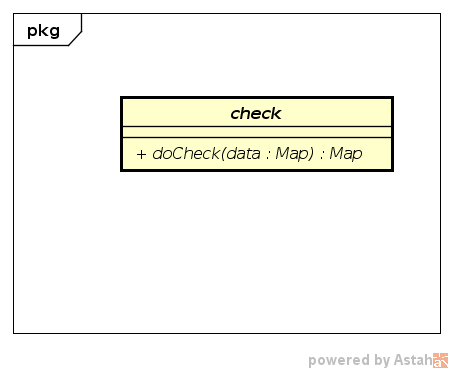
\includegraphics[width=0.6\textwidth]{img/single-check}
   \caption{{Diagramma per check in Checks}}
\end{figure}
\FloatBarrier
\textbf{Descrizione}\\
Classe concreta di concreteCheck che serve per effettuare controlli sui dati.
\textbf{Metodi:}
\begin{itemize}\item +doCheck() : boolean \\Ritorna il risultato di un controllo, true se positivo false se negativo.\end{itemize} 


\textbf{Applicazioni}\\
Interfaccia che viene utilizzata come rappresentazione di concreteCheck. 


\clearpage

\subsubsection{checkCreator}
\textbf{Componente:}  Monolith::Database::informationStorage::Checks\\
   \FloatBarrier
   \begin{figure}[ht]
   \centering
   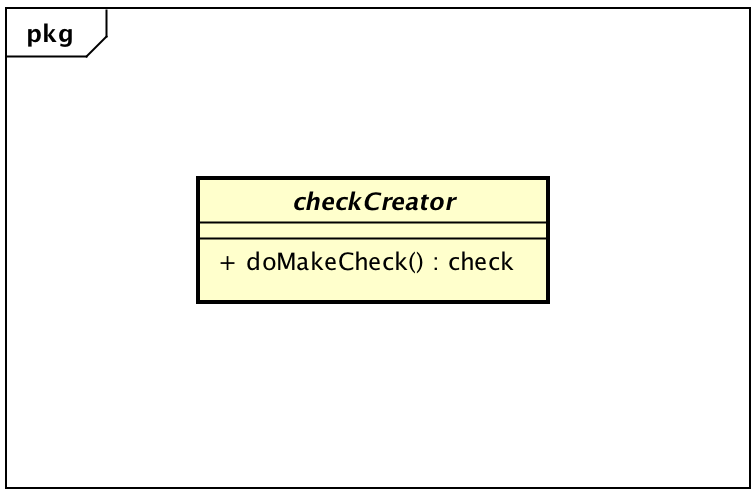
\includegraphics[width=0.6\textwidth]{img/single-checkCreator}
   \caption{{Diagramma per checkCreator in Checks}}
\end{figure}
\FloatBarrier
\textbf{Descrizione}\\
Classe astratta di concreteCheckCreator. \\\\ 
\textbf{Metodi:} \begin{itemize}\item +doMakeCheck() : check \\Ritorna un'istanza di check.\end{itemize} 


\textbf{Applicazioni}\\
Viene utilizzata quando viene richiesto un controllo. 


\clearpage

\subsubsection{concreteCheck}
\textbf{Componente:}  Monolith::Database::informationStorage::Checks\\
   \FloatBarrier
   \begin{figure}[ht]
   \centering
   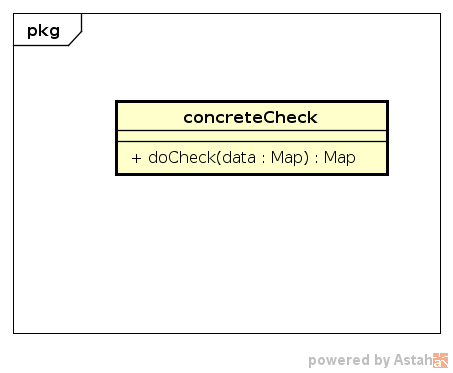
\includegraphics[width=0.6\textwidth]{img/single-concreteCheck}
   \caption{{Diagramma per concreteCheck in Checks}}
\end{figure}
\FloatBarrier
\textbf{Descrizione}\\
Classe che effettua un controllo e ne ritorna il risultato. \\\\
\textbf{Metodi:} \begin{itemize} \item +doCheck() : bool \\Ritorna il risultato di un controllo, true se positivo false se negativo.\end{itemize} 


\textbf{Applicazioni}\\
Viene utilizzata per effettuare controlli sui dati. 


\clearpage

\subsubsection{checkDiscriminator}
\textbf{Componente:}  Monolith::Database::informationStorage::Checks\\
   \FloatBarrier
   \begin{figure}[ht]
   \centering
   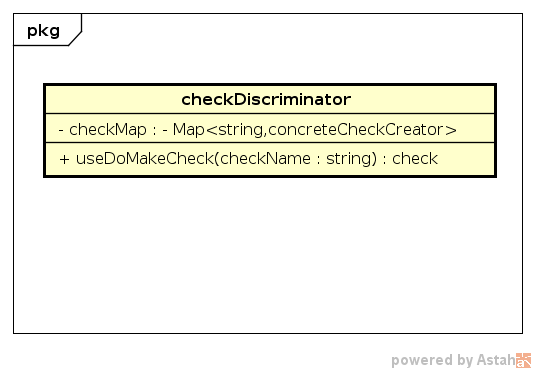
\includegraphics[width=0.6\textwidth]{img/single-checkDiscriminator}
   \caption{{Diagramma per checkDiscriminator in Checks}}
\end{figure}
\FloatBarrier
\textbf{Descrizione}\\
Classe che effettua il controllo in base alla stringa considerata. \\\\ 
\textbf{Attributi:} \begin{itemize}\item -checkMap : Map$<$ string , concreteCheckCreator $>$ \\Struttura che mappa il nome del check con l'istanza del checkCreator.\end{itemize}
\textbf{Metodi:} \begin{itemize}
\item +useDoMakeCheck(checkName : string) : bool \\Ritorna il risultato del controllo corrispondete alla stringa passata.
\end{itemize} 


\textbf{Applicazioni}\\
Viene utilizzata quando viene richiesto un controllo. 


\clearpage

\subsubsection{concreteCheckCreator}
\textbf{Componente:}  Monolith::Database::informationStorage::Checks\\
   \FloatBarrier
   \begin{figure}[ht]
   \centering
   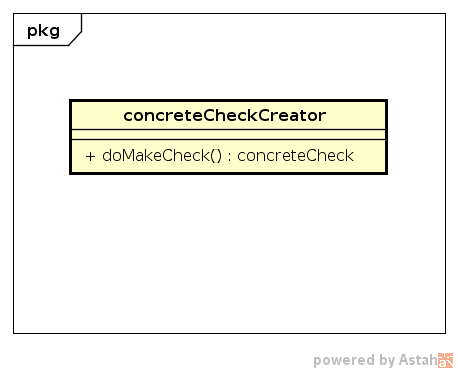
\includegraphics[width=0.6\textwidth]{img/single-concreteCheckCreator}
   \caption{{Diagramma per concreteCheckCreator in Checks}}
\end{figure}
\FloatBarrier
\textbf{Descrizione}\\
Classe che rappresenta istanze concrete di tipo check. \\\\ 
\textbf{Metodi:} \begin{itemize}\item +doMakeCheck() : concreteCheck \\Ritorna un'istanza di concreteCheck.\end{itemize} 


\textbf{Applicazioni}\\
Viene utilizzata per creare istanze di controlli. 


\clearpage

\subsubsection{Bubble}
\textbf{Componente:}  Monolith::UI::Bubbles\\
   \FloatBarrier
   \begin{figure}[ht]
   \centering
   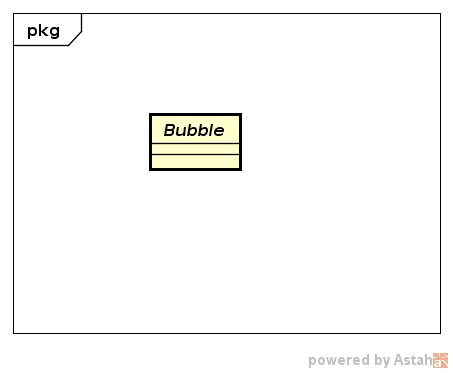
\includegraphics[width=0.6\textwidth]{img/single-Bubble}
   \caption{{Diagramma per Bubble in Bubbles}}
\end{figure}
\FloatBarrier
\textbf{Descrizione}\\
Classe Astratta di ConcreteBubble. 


\textbf{Applicazioni}\\
Viene utilizzata come interfaccia generica di bolla. 


\clearpage

\subsubsection{BubbleConfig}
\textbf{Componente:}  Monolith::UI::Bubbles\\
   \FloatBarrier
   \begin{figure}[ht]
   \centering
   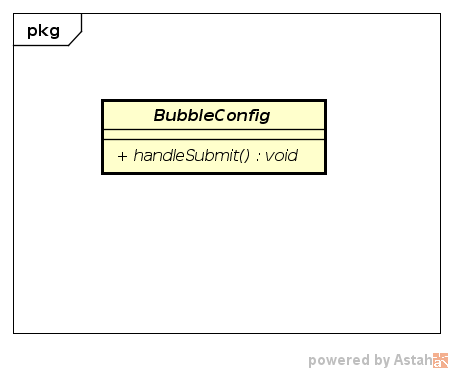
\includegraphics[width=0.6\textwidth]{img/single-BubbleConfig}
   \caption{{Diagramma per BubbleConfig in Bubbles}}
\end{figure}
\FloatBarrier
\textbf{Descrizione}\\
Classe Astratta di ConcreteBubbleConfig. 


\textbf{Applicazioni}\\
Interfaccia che viene utilizzata come rappresentazione di ConcreteBubbleConfig. 


\clearpage

\subsubsection{bubbleCreator}
\textbf{Componente:}  Monolith::UI::Bubbles\\
   \FloatBarrier
   \begin{figure}[ht]
   \centering
   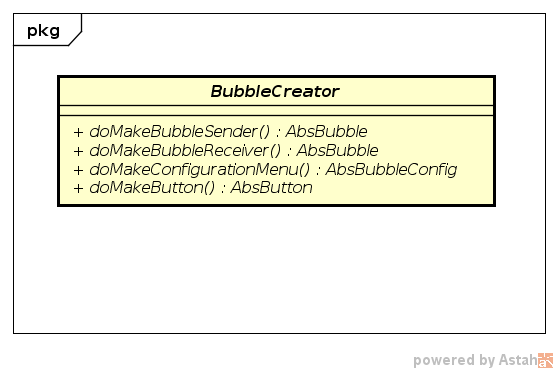
\includegraphics[width=0.6\textwidth]{img/single-bubbleCreator}
   \caption{{Diagramma per bubbleCreator in Bubbles}}
\end{figure}
\FloatBarrier
\textbf{Descrizione}\\
Classe astratta di concreteBubbleCreator. \\\\ 
\textbf{Metodi:} \\
\begin{itemize}\item +doMakeBubbleSender() : ConcreteBubble \\Ritorna il componente React per visualizzare una bolla inviata.\item +doMakeBubbleReceiver() : ConcreteBubble \\Ritorna il componente React per visualizzare una bolla ricevuta.\item +doMakeConfigurationMenu() : ConcreteBubbleConfig \\Ritorna il componente React per visualizzare il menù di creazione di una bolla da inviare.\item +doMakeButton() : ConcreteBubbleCreationButton \\Ritorna il componente React per visualizzare il bottone di creazione del menù di configurazione di una bolla da inviare.

\end{itemize} 


\textbf{Applicazioni}\\
Interfaccia che viene utilizzata come rappresentazione di concreteBubbleCreator. 


\clearpage

\subsubsection{ConcreteBubble}
\textbf{Componente:}  Monolith::UI::Bubbles\\
   \FloatBarrier
   \begin{figure}[ht]
   \centering
   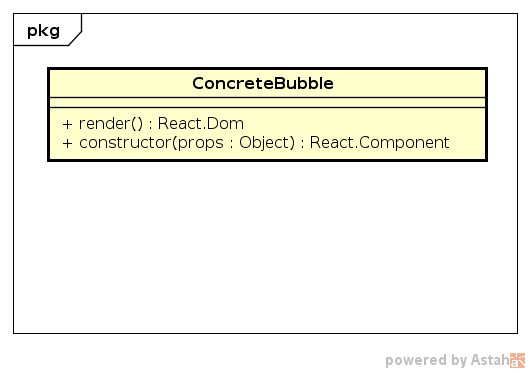
\includegraphics[width=0.6\textwidth]{img/single-ConcreteBubble}
   \caption{{Diagramma per ConcreteBubble in Bubbles}}
\end{figure}
\FloatBarrier
\textbf{Descrizione}\\
Classe React che rappresenta una bolla inviata o ricevuta.

\textbf{Metodi:} \begin{itemize}\item +constructor(props : Object) : React.Component \\Costruttore della sottoclasse di React.Component in cui è necessario chiamare super (props) ed è possibile inizializzare lo stato per i dati soggetti a cambiamento. 

\item +render() : React.DOM \\Metodo che esamina this.props e this.state e restituisce un singolo elemento React che può essere una rappresentazione di un componente DOM nativo o un altro componente composito.\end{itemize} 


\textbf{Applicazioni}\\
Viene utilizzata da concreteBubbleCreator per creare una bolla inviata o ricevuta dai dati recuperati da meteor. 


\clearpage

\subsubsection{bubbleDiscriminator}
\textbf{Componente:}  Monolith::UI::Bubbles\\
   \FloatBarrier
   \begin{figure}[ht]
   \centering
   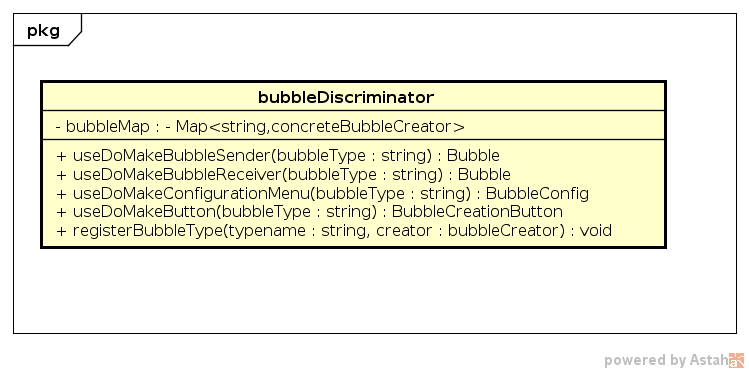
\includegraphics[width=0.6\textwidth]{img/single-bubbleDiscriminator}
   \caption{{Diagramma per bubbleDiscriminator in Bubbles}}
\end{figure}
\FloatBarrier
\textbf{Descrizione}\\
Classe che contiene i metodi che ritornano le funzionalità necessarie per la rappresentazione delle bolle.

\textbf{Attributi:}
\begin{itemize}\item -bubbleMap : Map$<$ string,concreteBubbleCreator$>$ \\Struttura che mappa il nome di una bolla con l'istanza di concreteBubbleCreator per quella bolla.\end{itemize}
\textbf{Metodi:} \begin{itemize}\item +useDoMakeBubbleSender( bubbleType: string) : ConcreteBubble \\Ritorna il componente React della stringa passata come parametro per visualizzare una bolla inviata.\item +useDoMakeBubbleReceiver( bubbleType: string) : ConcreteBubble \\Ritorna il componente React della stringa passata come parametro per visualizzare una bolla ricevuta.\item +useDoMakeBubbleConfigurationMenu( bubbleType: string) : ConcreteBubbleConfig \\Ritorna il componente React della stringa passata come parametro per visualizzare il menù di creazione di una bolla da inviare.\item  +useDoMakeButton( bubbleType: string) : ConcreteBubbleCreationButton \\ Ritorna il componente React della stringa passata come parametro per visualizzare il bottone di creazione del menù di configurazione di una bolla da inviare.

\end{itemize} 


\textbf{Applicazioni}\\
Viene utilizzata quando si deve creare una nuova bolla, ritornando l'oggetto della bolla appena selezionata. 


\clearpage

\subsubsection{BubbleCreationButton}
\textbf{Componente:}  Monolith::UI::Bubbles\\
   \FloatBarrier
   \begin{figure}[ht]
   \centering
   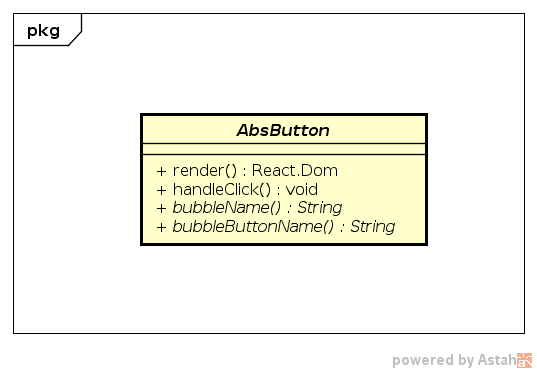
\includegraphics[width=0.6\textwidth]{img/single-BubbleCreationButton}
   \caption{{Diagramma per BubbleCreationButton in Bubbles}}
\end{figure}
\FloatBarrier
\textbf{Descrizione}\\
Classe Astratta di ConcreteBubbleCreationButton. 


\textbf{Applicazioni}\\
Interfaccia che viene utilizzata come rappresentazione di ConcreteBubbleCreationButton. 


\clearpage

\subsubsection{ConcreteBubbleConfig}
\textbf{Componente:}  Monolith::UI::Bubbles\\
   \FloatBarrier
   \begin{figure}[ht]
   \centering
   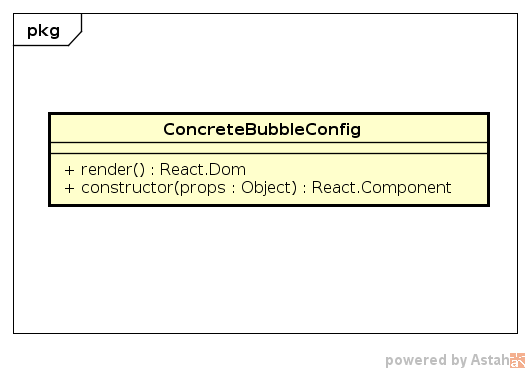
\includegraphics[width=0.6\textwidth]{img/single-ConcreteBubbleConfig}
   \caption{{Diagramma per ConcreteBubbleConfig in Bubbles}}
\end{figure}
\FloatBarrier
\textbf{Descrizione}\\
Classe che rappresenta il menù di creazione di una bolla.


\textbf{Metodi:} \begin{itemize}\item +constructor(props : Object) : React.Component \\Costruttore della sottoclasse di React.Component in cui è necessario chiamare super (props) ed è possibile inizializzare lo stato per i dati soggetti a cambiamento. 

\item +render() : React.DOM \\Metodo che esamina this.props e this.state e restituisce un singolo elemento React che può essere una rappresentazione di un componente DOM nativo o un altro componente composito.\end{itemize} 


\textbf{Applicazioni}\\
Viene utilizzata da concreteBubbleCreator per creare un istanza del menù di creazione di una bolla. 


\clearpage

\subsubsection{concreteBubbleCreator}
\textbf{Componente:}  Monolith::UI::Bubbles\\
   \FloatBarrier
   \begin{figure}[ht]
   \centering
   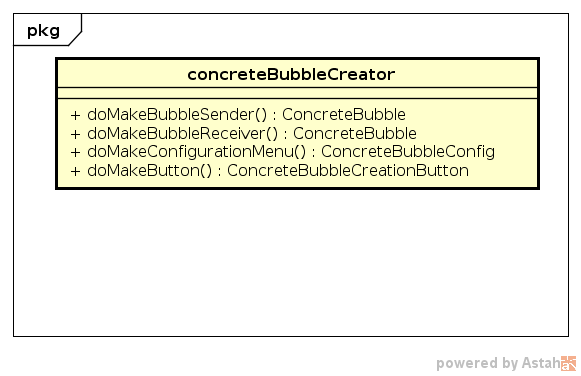
\includegraphics[width=0.6\textwidth]{img/single-concreteBubbleCreator}
   \caption{{Diagramma per concreteBubbleCreator in Bubbles}}
\end{figure}
\FloatBarrier
\textbf{Descrizione}\\
Classe che contiene i factory method utilizzati per la creazione degli oggetti concreti di tipo Bubble, BubbleConfig e BubbleCreationButton.

\textbf{Metodi:} \begin{itemize}
\item +doMakeBubbleSender() : ConcreteBubble \\Ritorna il componente React per visualizzare una bolla inviata.\item +doMakeBubbleReceiver() : ConcreteBubble \\Ritorna il componente React per visualizzare una bolla ricevuta.\item +doMakeConfigurationMenu() : ConcreteBubbleConfig \\Ritorna il componente React per visualizzare il menù di creazione di una bolla da inviare.\item +doMakeButton() : ConcreteBubbleCreationButton \\Ritorna il componente React per visualizzare il bottone di creazione del menù di configurazione di una bolla da inviare.


\end{itemize} 


\textbf{Applicazioni}\\
Viene utilizzata da bubbleDiscriminator per creare le bolle ricevute e inviate, i menù di configurazione delle bolle e i bottoni per aprire il menù di configurazione delle bolle. 


\clearpage

\subsubsection{ConcreteBubbleCreationButton}
\textbf{Componente:}  Monolith::UI::Bubbles\\
   \FloatBarrier
   \begin{figure}[ht]
   \centering
   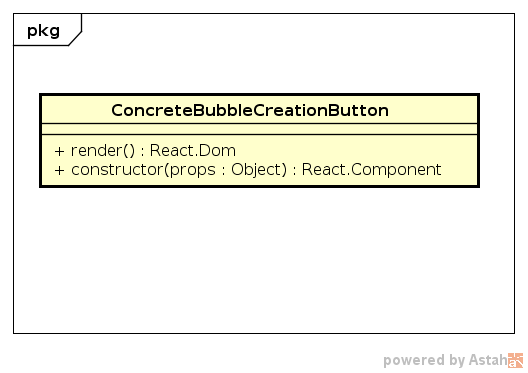
\includegraphics[width=0.6\textwidth]{img/single-ConcreteBubbleCreationButton}
   \caption{{Diagramma per ConcreteBubbleCreationButton in Bubbles}}
\end{figure}
\FloatBarrier
\textbf{Descrizione}\\
Classe che rappresenta il bottone per aprire il menù di creazione di una bolla.


\textbf{Metodi:} \begin{itemize}\item +constructor(props : Object) : React.Component \\Costruttore della sottoclasse di React.Component in cui è necessario chiamare super (props) ed è possibile inizializzare lo stato per i dati soggetti a cambiamento. 

\item +render() : React.DOM \\Metodo che esamina this.props e this.state e restituisce un singolo elemento React che può essere una rappresentazione di un componente DOM nativo o un altro componente composito.\end{itemize} 


\textbf{Applicazioni}\\
Viene utilizzata da concreteBubbleCreator per creare un istanza di un bottone nel menù di selezione di una bolla. 


\clearpage

\subsubsection{SideArea1}
\textbf{Componente:}  Monolith::UI::SideAreas::SideArea1\_pkg\\
   \FloatBarrier
   \begin{figure}[ht]
   \centering
   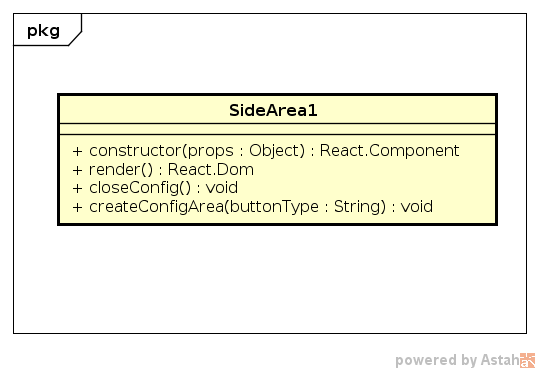
\includegraphics[width=0.6\textwidth]{img/single-SideArea1}
   \caption{{Diagramma per SideArea1 in SideArea1\_pkg}}
\end{figure}
\FloatBarrier
\textbf{Descrizione}\\
Classe che rappresenta il componente React per la visualizzazione del contenuto della prima area laterale. \\\\ 
\textbf{Metodi:} \begin{itemize}\item +constructor(props : Object) : React.Component \\Costruttore della sottoclasse di React.Component in cui è necessario chiamare super (props) ed è possibile inizializzare lo stato per i dati soggetti a cambiamento.\item +render() : React.DOM \\Metodo che esamina this.props e this.state e restituisce un singolo elemento React che può essere una rappresentazione di un componente DOM nativo o un altro componente composito.\end{itemize} 


\textbf{Applicazioni}\\
Viene utilizzata all'apertura della prima area laterale per visualizzare il menù di creazione delle bolle e lo storico delle bolle inviate. 


\clearpage

\subsubsection{SentBubbleHistory}
\textbf{Componente:}  Monolith::UI::SideAreas::SideArea1\_pkg\\
   \FloatBarrier
   \begin{figure}[ht]
   \centering
   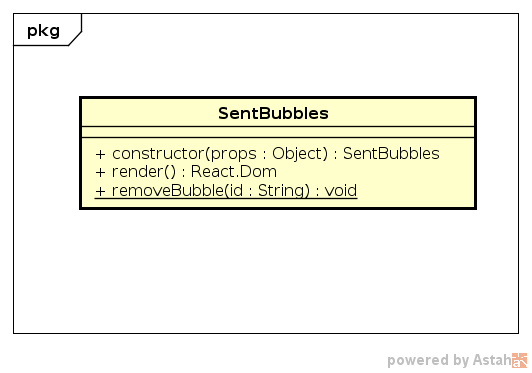
\includegraphics[width=0.6\textwidth]{img/single-SentBubbleHistory}
   \caption{{Diagramma per SentBubbleHistory in SideArea1\_pkg}}
\end{figure}
\FloatBarrier
\textbf{Descrizione}\\
Classe che rappresenta il componente React per la visualizzazione dello storico delle bolle inviate.

\textbf{Metodi:} \begin{itemize}\item +constructor(props : Object) : React.Component \\Costruttore della sottoclasse di React.Component in cui è necessario chiamare super (props) ed è possibile inizializzare lo stato per i dati soggetti a cambiamento.\item +render() : React.DOM \\Metodo che esamina this.props e this.state e restituisce un singolo elemento React che può essere una rappresentazione di un componente DOM nativo o un altro componente composito.\end{itemize} 


\textbf{Applicazioni}\\
Viene utilizzata dalla SideArea1 per la visualizzazione dello storico delle bolle inviate. 


\clearpage

\subsubsection{BubbleCreationMenu}
\textbf{Componente:}  Monolith::UI::SideAreas::SideArea1\_pkg\\
   \FloatBarrier
   \begin{figure}[ht]
   \centering
   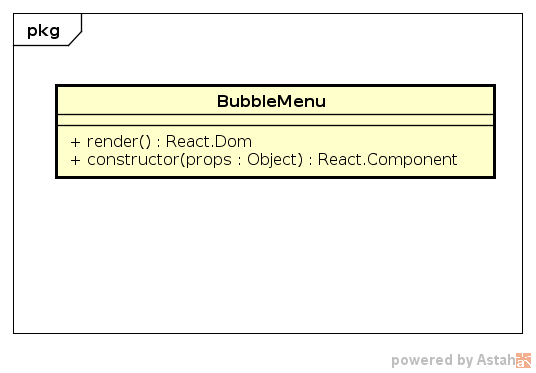
\includegraphics[width=0.6\textwidth]{img/single-BubbleCreationMenu}
   \caption{{Diagramma per BubbleCreationMenu in SideArea1\_pkg}}
\end{figure}
\FloatBarrier
\textbf{Descrizione}\\
Classe che rappresenta il componente React per la configurazione delle bolle.
\textbf{Metodi:} \begin{itemize}\item +constructor(props : Object) : React.Component \\Costruttore della sottoclasse di React.Component in cui è necessario chiamare super (props) ed è possibile inizializzare lo stato per i dati soggetti a cambiamento.\item +render() : React.DOM \\Metodo che esamina this.props e this.state e restituisce un singolo elemento React che può essere una rappresentazione di un componente DOM nativo o un altro componente composito.\end{itemize} 


\textbf{Applicazioni}\\
Viene utilizzata dalla SideArea1 per la visualizzazione del menù di creazione delle bolle. 


\clearpage

\subsubsection{SideArea2}
\textbf{Componente:}  Monolith::UI::SideAreas::SideArea2\_pkg\\
   \FloatBarrier
   \begin{figure}[ht]
   \centering
   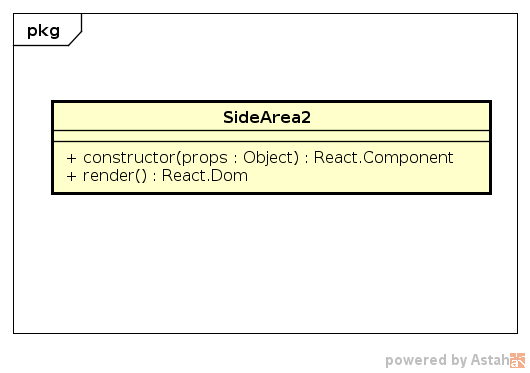
\includegraphics[width=0.6\textwidth]{img/single-SideArea2}
   \caption{{Diagramma per SideArea2 in SideArea2\_pkg}}
\end{figure}
\FloatBarrier
\textbf{Descrizione}\\
Classe che rappresenta il componente React per la visualizzazione del contenuto della seconda area laterale. \\\\
\textbf{Metodi:} \begin{itemize}\item +constructor(props : Object) : React.Component \\Costruttore della sottoclasse di React.Component in cui è necessario chiamare super (props) ed è possibile inizializzare lo stato per i dati soggetti a cambiamento.\item +render() : React.DOM \\Metodo che esamina this.props e this.state e restituisce un singolo elemento React che può essere una rappresentazione di un componente DOM nativo o un altro componente composito.

\end{itemize} 


\textbf{Applicazioni}\\
Viene utilizzata all'apertura della seconda area laterale per visualizzare dello storico delle bolle ricevute. 


\clearpage

\subsubsection{ReceivedBubbleHistory}
\textbf{Componente:}  Monolith::UI::SideAreas::SideArea2\_pkg\\
   \FloatBarrier
   \begin{figure}[ht]
   \centering
   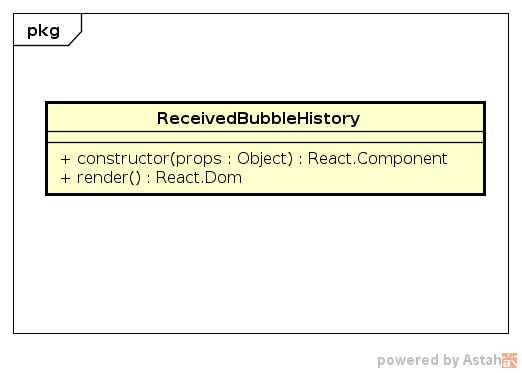
\includegraphics[width=0.6\textwidth]{img/single-ReceivedBubbleHistory}
   \caption{{Diagramma per ReceivedBubbleHistory in SideArea2\_pkg}}
\end{figure}
\FloatBarrier
\textbf{Descrizione}\\
Classe che rappresenta il componente React per la visualizzazione dello storico delle bolle ricevute. \\\\
\textbf{Metodi:} \begin{itemize}\item +constructor(props : Object) : React.Component \\Costruttore della sottoclasse di React.Component in cui è necessario chiamare super (props) ed è possibile inizializzare lo stato per i dati soggetti a cambiamento.\item +render() : React.DOM \\Metodo che esamina this.props e this.state e restituisce un singolo elemento React che può essere una rappresentazione di un componente DOM nativo o un altro componente composito.\end{itemize} 


\textbf{Applicazioni}\\
Viene utilizzata dalla SideArea2 per la visualizzazione dello storico delle bolle ricevute. 


\clearpage

\subsubsection{VerticalLayout}
\textbf{Componente:}  Monolith::UI::UI-Layouts\\
   \FloatBarrier
   \begin{figure}[ht]
   \centering
   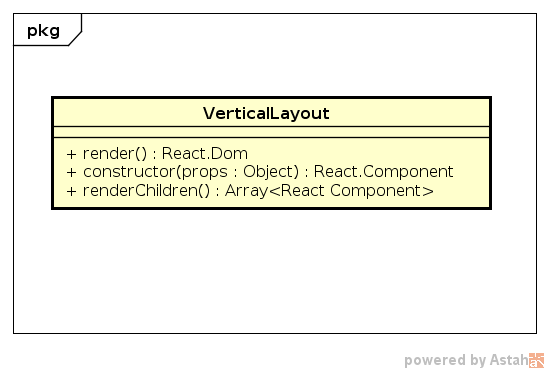
\includegraphics[width=0.6\textwidth]{img/single-VerticalLayout}
   \caption{{Diagramma per VerticalLayout in UI-Layouts}}
\end{figure}
\FloatBarrier
\textbf{Descrizione}\\
Classe contenitore che dispone i componenti contenuti uno sotto l'altro \\\\
\textbf{Metodi:} \begin{itemize}\item +constructor(props : Object) : React.Component \\Costruttore della sottoclasse di React.Component in cui è necessario chiamare super (props) ed è possibile inizializzare lo stato per i dati soggetti a cambiamento.\item +render() : React.DOM \\Metodo che esamina this.props e this.state e restituisce un singolo elemento React che può essere una rappresentazione di un componente DOM nativo o un altro componente composito.\end{itemize} 


\textbf{Applicazioni}\\
Utilizzata per assegnare l'attributo className bootstrap a tutti i componenti figli, in modo che vengano visualizzati allineati in verticale con la dimensione adeguata. 


\clearpage

\subsubsection{ContainedElement}
\textbf{Componente:}  Monolith::UI::UI-Layouts\\
   \FloatBarrier
   \begin{figure}[ht]
   \centering
   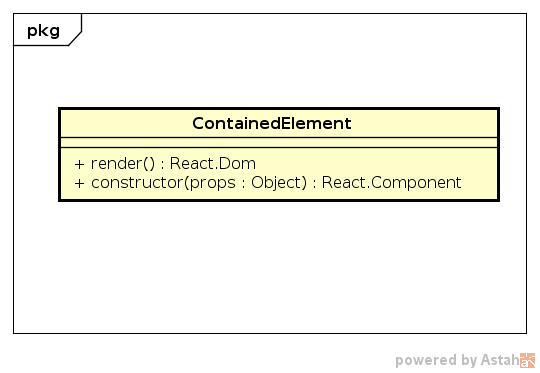
\includegraphics[width=0.6\textwidth]{img/single-ContainedElement}
   \caption{{Diagramma per ContainedElement in UI-Layouts}}
\end{figure}
\FloatBarrier
\textbf{Descrizione}\\
Classe che rappresenta un oggetto figlio dei Layout \\\\
\textbf{Metodi:} \begin{itemize}\item +constructor(props : Object) : React.Component \\Costruttore della sottoclasse di React.Component in cui è necessario chiamare super (props) ed è possibile inizializzare lo stato per i dati soggetti a cambiamento. \item +render() : React.DOM \\Metodo che esamina this.props e this.state e restituisce un singolo elemento React che può essere una rappresentazione di un componente DOM nativo o un altro componente composito.\end{itemize} 


\textbf{Applicazioni}\\
Viene utilizzata dalle classi HorizontalLayout, VerticalLayout e ConditionalRendering per contenere un componente generico 


\clearpage

\subsubsection{HorizontalLayout}
\textbf{Componente:}  Monolith::UI::UI-Layouts\\
   \FloatBarrier
   \begin{figure}[ht]
   \centering
   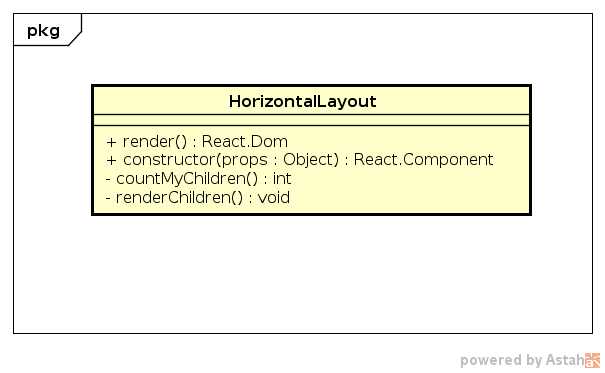
\includegraphics[width=0.6\textwidth]{img/single-HorizontalLayout}
   \caption{{Diagramma per HorizontalLayout in UI-Layouts}}
\end{figure}
\FloatBarrier
\textbf{Descrizione}\\
Classe contenitore che dispone i componenti contenuti in orizzontale. \\\\
\textbf{Metodi:} \begin{itemize}\item +constructor(props : Object) : React.Component \\Costruttore della sottoclasse di React.Component in cui è necessario chiamare super (props) ed è possibile inizializzare lo stato per i dati soggetti a cambiamento.\item +render() : React.DOM \\Metodo che esamina this.props e this.state e restituisce un singolo elemento React che può essere una rappresentazione di un componente DOM nativo o un altro componente composito.\item +countMyChildren() : int \\Metodo che ritorna un intero contente il numero di componenti figli, utilizzato per impostare la classe bootstrap corretta.\end{itemize} 


\textbf{Applicazioni}\\
Utilizzata per assegnare l'attributo className bootstrap a tutti i componenti figli, in modo che vengano visualizzati allineati in orizzontale con la dimensione adeguata. 


\clearpage

\subsubsection{ConditionalRendering}
\textbf{Componente:}  Monolith::UI::UI-Layouts\\
   \FloatBarrier
   \begin{figure}[ht]
   \centering
   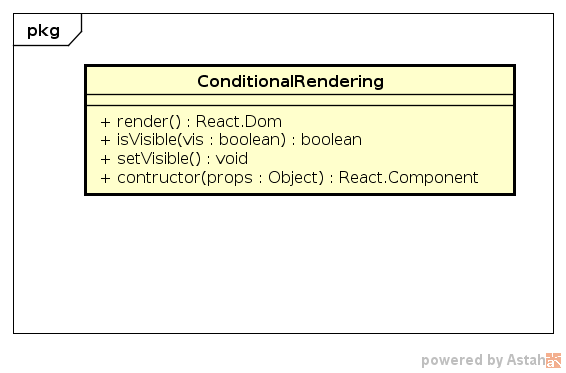
\includegraphics[width=0.6\textwidth]{img/single-ConditionalRendering}
   \caption{{Diagramma per ConditionalRendering in UI-Layouts}}
\end{figure}
\FloatBarrier
\textbf{Descrizione}\\
Classe che fornisce i metodi per nascondere un componente contenuto all'esecuzione di un suo metodo \\\\
\textbf{Metodi:} \\
\begin{itemize}\item +constructor(props : Object) : React.Component \\Costruttore della sottoclasse di React.Component in cui è necessario chiamare super (props) ed è possibile inizializzare lo stato per i dati soggetti a cambiamento.\item +setVisible(vis : boolean): void \\Imposta l'attributo che indica se il componente è visibile o meno in base al valore di vis.\item +isVisible() : boolean \\Metodo che ritorna true se il componente è visibile altrimenti ritorna false.\item +setVisible( vis : boolean ) : void \\Imposta l'attributo che indica se il componente è visibile o meno in base al valore del parametro.\item +isVisible() : bool \\Metodo che ritorna true se il componente è visibile altrimenti ritorna false.\item +render() : React.DOM \\Metodo che esamina this.props e this.state e restituisce un singolo elemento React che può essere una rappresentazione di un componente DOM nativo o un altro componente composito.\end{itemize} 


\textbf{Applicazioni}\\
Viene utilizzata per nascondere un componente a necessità. 


\clearpage

\subsubsection{Image}
\textbf{Componente:}  Monolith::UI::UI-SingleComponents\\
   \FloatBarrier
   \begin{figure}[ht]
   \centering
   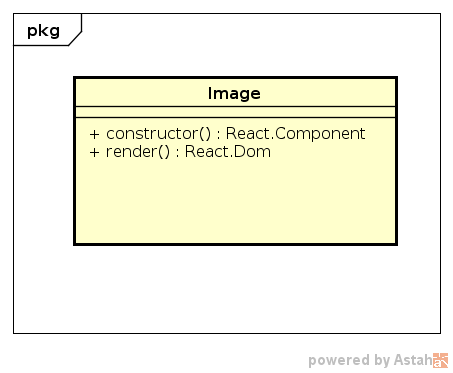
\includegraphics[width=0.6\textwidth]{img/single-Image}
   \caption{{Diagramma per Image in UI-SingleComponents}}
\end{figure}
\FloatBarrier
\textbf{Descrizione}\\
Componente React che rappresenta un'immagine. \\\\
\textbf{Metodi:} \begin{itemize}\item +constructor(props : Object) : React.Component \\Costruttore della sottoclasse di React.Component in cui è necessario chiamare super (props) ed è possibile inizializzare lo stato per i dati soggetti a cambiamento.\item +render() : React.DOM \\Metodo che esamina this.props e this.state e restituisce un singolo elemento React che può essere una rappresentazione di un componente DOM nativo o un altro componente composito.\end{itemize} 


\textbf{Applicazioni}\\
Viene utilizzato per costruire le interfacce grafiche delle bolle. 


\clearpage

\subsubsection{ComboBox}
\textbf{Componente:}  Monolith::UI::UI-SingleComponents\\
   \FloatBarrier
   \begin{figure}[ht]
   \centering
   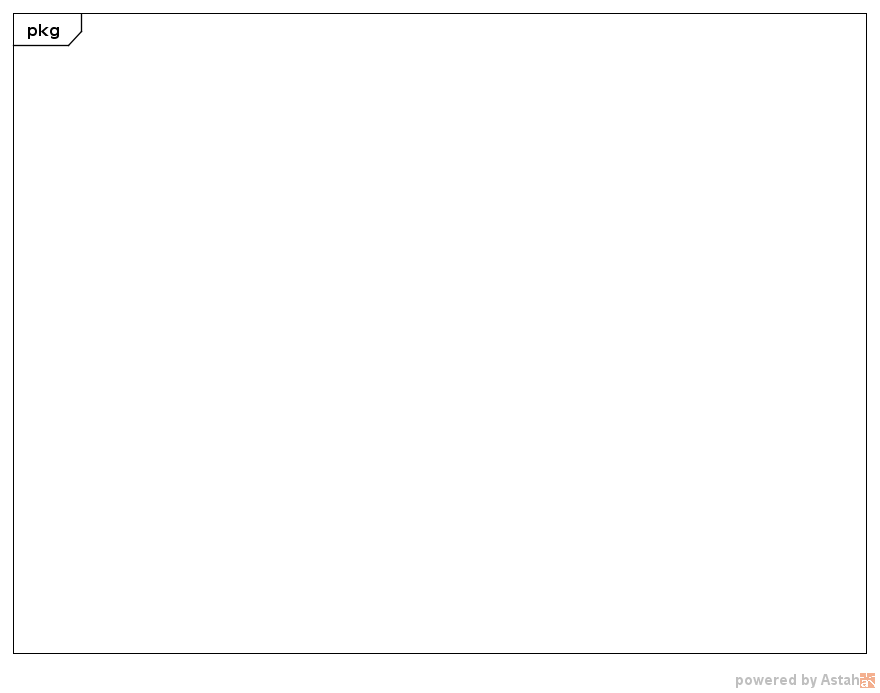
\includegraphics[width=0.6\textwidth]{img/single-ComboBox}
   \caption{{Diagramma per ComboBox in UI-SingleComponents}}
\end{figure}
\FloatBarrier
\textbf{Descrizione}\\
Componente React che rappresenta un combobox. \\\\
\textbf{Metodi:} \begin{itemize}\item +constructor(props : Object) : React.Component \\Costruttore della sottoclasse di React.Component in cui è necessario chiamare super (props) ed è possibile inizializzare lo stato per i dati soggetti a cambiamento.\item +optChange(event : String) : void  \\Comunica l’opzione selezionata tramite il metodo del genitore. \item +render() : React.DOM \\Metodo che esamina this.props e this.state e restituisce un singolo elemento React che può essere una rappresentazione di un componente DOM nativo o un altro componente composito.\end{itemize} 


\textbf{Applicazioni}\\
Viene utilizzato per costruire le interfacce grafiche delle bolle. 


\clearpage

\subsubsection{LineEdit}
\textbf{Componente:}  Monolith::UI::UI-SingleComponents\\
   \FloatBarrier
   \begin{figure}[ht]
   \centering
   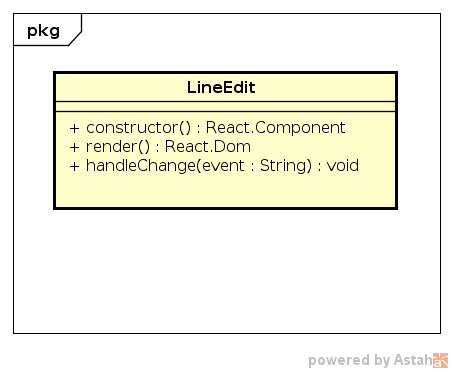
\includegraphics[width=0.6\textwidth]{img/single-LineEdit}
   \caption{{Diagramma per LineEdit in UI-SingleComponents}}
\end{figure}
\FloatBarrier
\textbf{Descrizione}\\
Componente React che rappresenta un input di testo. \\\\
\textbf{Metodi:} \begin{itemize}\item +constructor(props : Object) : React.Component \\Costruttore della sottoclasse di React.Component in cui è necessario chiamare super (props) ed è possibile inizializzare lo stato per i dati soggetti a cambiamento.\item +handleChange(event : String) : void  \\Comunica l’opzione selezionata tramite il metodo del genitore. \item +render() : React.DOM \\Metodo che esamina this.props e this.state e restituisce un singolo elemento React che può essere una rappresentazione di un componente DOM nativo o un altro componente composito.\end{itemize} 


\textbf{Applicazioni}\\
Viene utilizzato per costruire le interfacce grafiche delle bolle. 


\clearpage

\subsubsection{LabelEdit}
\textbf{Componente:}  Monolith::UI::UI-SingleComponents\\
   \FloatBarrier
   \begin{figure}[ht]
   \centering
   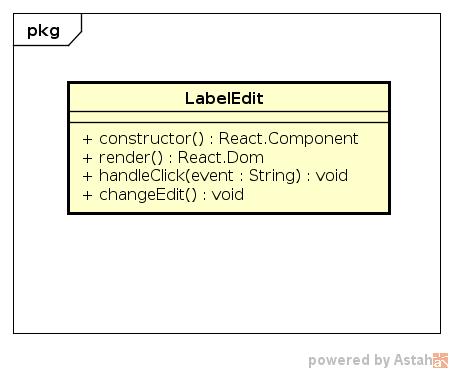
\includegraphics[width=0.6\textwidth]{img/single-LabelEdit}
   \caption{{Diagramma per LabelEdit in UI-SingleComponents}}
\end{figure}
\FloatBarrier
\textbf{Descrizione}\\
Componente React che rappresenta una label che quando viene cliccata diventa un campo di inserimento testo. \\\\
\textbf{Metodi:} \begin{itemize}\item +constructor(props : Object) : React.Component \\Costruttore della sottoclasse di React.Component in cui è necessario chiamare super (props) ed è possibile inizializzare lo stato per i dati soggetti a cambiamento.\item +handleClick(event : String) : void  \\Viene invocato il metodo del genitore per trasferirvi il cambiamento di stato\item +changeEdit() : void \\Cambia lo stato del componente rendendolo (o meno) modificabile\item +render() : React.DOM \\Metodo che esamina this.props e this.state e restituisce un singolo elemento React che può essere una rappresentazione di un componente DOM nativo o un altro componente composito.\end{itemize} 


\textbf{Applicazioni}\\
Viene utilizzato per costruire le interfacce grafiche delle bolle. 


\clearpage

\subsubsection{PushButton}
\textbf{Componente:}  Monolith::UI::UI-SingleComponents\\
   \FloatBarrier
   \begin{figure}[ht]
   \centering
   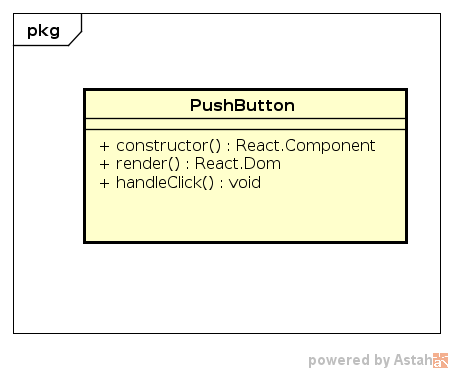
\includegraphics[width=0.6\textwidth]{img/single-PushButton}
   \caption{{Diagramma per PushButton in UI-SingleComponents}}
\end{figure}
\FloatBarrier
\textbf{Descrizione}\\
Componente React che rappresenta un pulsante cliccabile. \\\\
\textbf{Metodi:} \begin{itemize}\item +constructor(props : Object) : React.Component \\Costruttore della sottoclasse di React.Component in cui è necessario chiamare super (props) ed è possibile inizializzare lo stato per i dati soggetti a cambiamento.\item +handleClick(): void \\Viene invocato il metodo passato dal genitore\item +render() : React.DOM \\Metodo che esamina this.props e this.state e restituisce un singolo elemento React che può essere una rappresentazione di un componente DOM nativo o un altro componente composito.\end{itemize} 


\textbf{Applicazioni}\\
Viene utilizzato per costruire le interfacce grafiche delle bolle. 


\clearpage

\subsubsection{CheckButton}
\textbf{Componente:}  Monolith::UI::UI-SingleComponents\\
   \FloatBarrier
   \begin{figure}[ht]
   \centering
   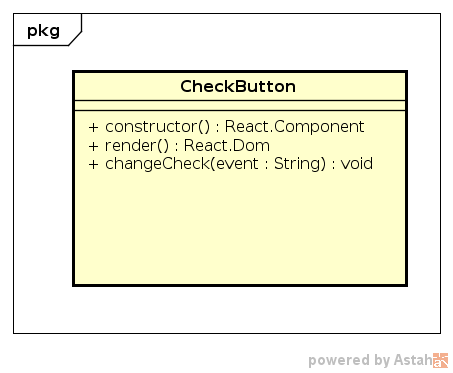
\includegraphics[width=0.6\textwidth]{img/single-CheckButton}
   \caption{{Diagramma per CheckButton in UI-SingleComponents}}
\end{figure}
\FloatBarrier
\textbf{Descrizione}\\
Componente React che rappresenta un elemento di checkbox. \\\\
\textbf{Metodi:} \begin{itemize}\item +constructor(props : Object) : React.Component \\Costruttore della sottoclasse di React.Component in cui è necessario chiamare super (props) ed è possibile inizializzare lo stato per i dati soggetti a cambiamento.\item +changeCheck(event : String) : void  \\Comunica l’opzione selezionata tramite il metodo del genitore. \item +render() : React.DOM \\Metodo che esamina this.props e this.state e restituisce un singolo elemento React che può essere una rappresentazione di un componente DOM nativo o un altro componente composito.\end{itemize} 


\textbf{Applicazioni}\\
Viene utilizzato per costruire le interfacce grafiche delle bolle. 


\clearpage

\subsubsection{ImageButton}
\textbf{Componente:}  Monolith::UI::UI-SingleComponents\\
   \FloatBarrier
   \begin{figure}[ht]
   \centering
   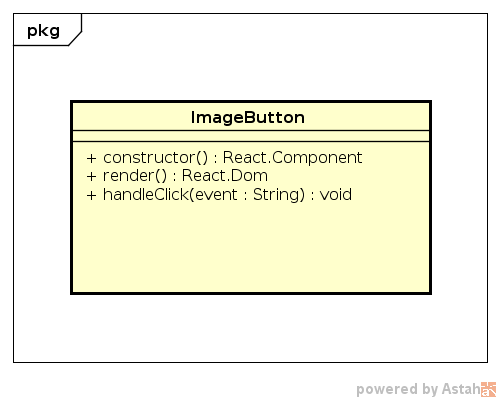
\includegraphics[width=0.6\textwidth]{img/single-ImageButton}
   \caption{{Diagramma per ImageButton in UI-SingleComponents}}
\end{figure}
\FloatBarrier
\textbf{Descrizione}\\
Componente React che rappresenta un immagine che funge da pulsante. \\\\
\textbf{Metodi:} \begin{itemize}\item +constructor(props : Object) : React.Component \\Costruttore della sottoclasse di React.Component in cui è necessario chiamare super (props) ed è possibile inizializzare lo stato per i dati soggetti a cambiamento.\item +handleClick(event : String) : void  \\Comunica l’opzione selezionata tramite il metodo del genitore. \item +render() : React.DOM \\Metodo che esamina this.props e this.state e restituisce un singolo elemento React che può essere una rappresentazione di un componente DOM nativo o un altro componente composito.\end{itemize} 


\textbf{Applicazioni}\\
Viene utilizzato per costruire le interfacce grafiche delle bolle. 


\clearpage

\subsubsection{CheckBoxList}
\textbf{Componente:}  Monolith::UI::UI-SingleComponents\\
   \FloatBarrier
   \begin{figure}[ht]
   \centering
   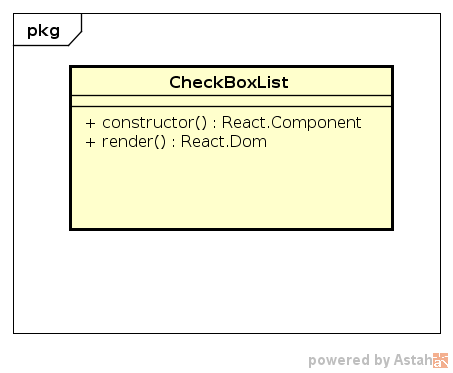
\includegraphics[width=0.6\textwidth]{img/single-CheckBoxList}
   \caption{{Diagramma per CheckBoxList in UI-SingleComponents}}
\end{figure}
\FloatBarrier
\textbf{Descrizione}\\
Componente React che rappresenta una lista di CheckBox. \\\\
\textbf{Metodi:} \begin{itemize}\item +constructor(props : Object) : React.Component \\Costruttore della sottoclasse di React.Component in cui è necessario chiamare super (props) ed è possibile inizializzare lo stato per i dati soggetti a cambiamento.\item +render() : React.DOM \\Metodo che esamina this.props e this.state e restituisce un singolo elemento React che può essere una rappresentazione di un componente DOM nativo o un altro componente composito.

\end{itemize} 


\textbf{Applicazioni}\\
Viene utilizzato per costruire le interfacce grafiche delle bolle. 


\clearpage

\subsubsection{LabelComboBox}
\textbf{Componente:}  Monolith::UI::UI-SingleComponents\\
   \FloatBarrier
   \begin{figure}[ht]
   \centering
   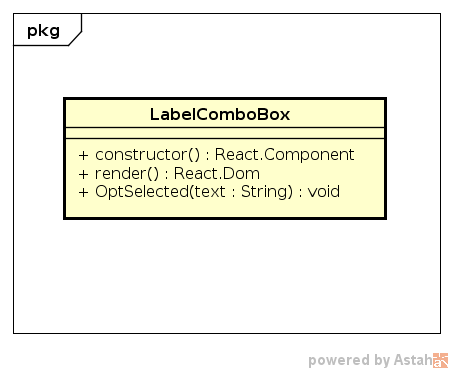
\includegraphics[width=0.6\textwidth]{img/single-LabelComboBox}
   \caption{{Diagramma per LabelComboBox in UI-SingleComponents}}
\end{figure}
\FloatBarrier
\textbf{Descrizione}\\
Componente React che rappresenta una lista di item selezionabile affiancata da una Label. \\\\
\textbf{Metodi:} \begin{itemize}\item +constructor(props : Object) : React.Component \\Costruttore della sottoclasse di React.Component in cui è necessario chiamare super (props) ed è possibile inizializzare lo stato per i dati soggetti a cambiamento.\item +OptSelected(text : String) : void \\ Comunica l’opzione selezionata tramite il metodo del genitore. \item +render() : React.DOM \\Metodo che esamina this.props e this.state e restituisce un singolo elemento React che può essere una rappresentazione di un componente DOM nativo o un altro componente composito.\end{itemize} 


\textbf{Applicazioni}\\
Viene utilizzato per costruire le interfacce grafiche delle bolle. 


\clearpage

\subsubsection{TextAreaButton}
\textbf{Componente:}  Monolith::UI::UI-SingleComponents\\
   \FloatBarrier
   \begin{figure}[ht]
   \centering
   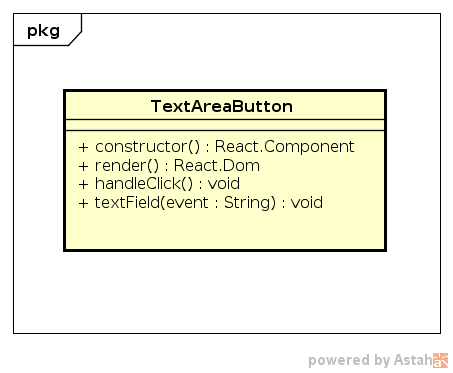
\includegraphics[width=0.6\textwidth]{img/single-TextAreaButton}
   \caption{{Diagramma per TextAreaButton in UI-SingleComponents}}
\end{figure}
\FloatBarrier
\textbf{Descrizione}\\
Componente React che rappresenta un'area di testo con un pulsante. \\\\
\textbf{Metodi:} \begin{itemize}\item +constructor(props : Object) : React.Component \\Costruttore della sottoclasse di React.Component in cui è necessario chiamare super (props) ed è possibile inizializzare lo stato per i dati soggetti a cambiamento.\item +textField(text : String) : void \\Comunica l’opzione selezionata tramite il metodo del genitore.\item +handleClick(event : String) : void  \\Comunica l’opzione selezionata tramite il metodo del genitore. \item +render() : React.DOM \\Metodo che esamina this.props e this.state e restituisce un singolo elemento React che può essere una rappresentazione di un componente DOM nativo o un altro componente composito.\end{itemize} 


\textbf{Applicazioni}\\
Viene utilizzato per costruire le interfacce grafiche delle bolle. 


\clearpage

\subsubsection{LabelPushButton}
\textbf{Componente:}  Monolith::UI::UI-SingleComponents\\
   \FloatBarrier
   \begin{figure}[ht]
   \centering
   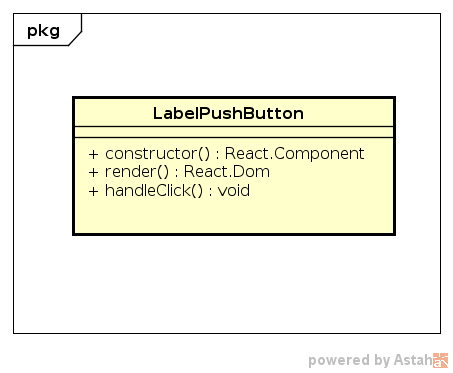
\includegraphics[width=0.6\textwidth]{img/single-LabelPushButton}
   \caption{{Diagramma per LabelPushButton in UI-SingleComponents}}
\end{figure}
\FloatBarrier
\textbf{Descrizione}\\
Componente React che rappresenta un Label affiancato da un bottone cliccabile. \\\\
\textbf{Metodi:} \begin{itemize}\item +constructor(props : Object) : React.Component \\Costruttore della sottoclasse di React.Component in cui è necessario chiamare super (props) ed è possibile inizializzare lo stato per i dati soggetti a cambiamento.\item +handleClick(event : String) : void  \\Comunica l’opzione selezionata tramite il metodo del genitore.\item +render() : React.DOM \\Metodo che esamina this.props e this.state e restituisce un singolo elemento React che può essere una rappresentazione di un componente DOM nativo o un altro componente composito.\end{itemize} 


\textbf{Applicazioni}\\
Viene utilizzato per costruire le interfacce grafiche delle bolle. 


\clearpage

\subsubsection{LineEditComboBox}
\textbf{Componente:}  Monolith::UI::UI-SingleComponents\\
   \FloatBarrier
   \begin{figure}[ht]
   \centering
   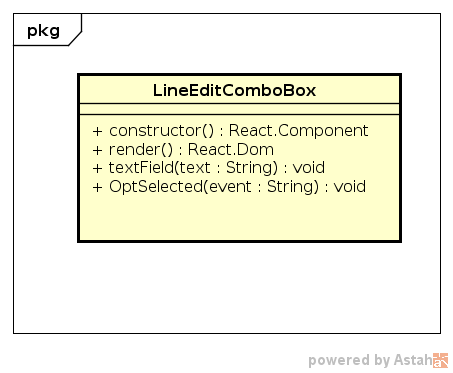
\includegraphics[width=0.6\textwidth]{img/single-LineEditComboBox}
   \caption{{Diagramma per LineEditComboBox in UI-SingleComponents}}
\end{figure}
\FloatBarrier
\textbf{Descrizione}\\
Componente React che rappresenta una LineEdit con a fianco un ComboBox. \\\\
\textbf{Metodi:} \begin{itemize}\item +constructor(props : Object) : React.Component \\Costruttore della sottoclasse di React.Component in cui è necessario chiamare super (props) ed è possibile inizializzare lo stato per i dati soggetti a cambiamento.\item +textField(text : String) : void \\Comunica il contenuto della textarea tramite il metodo del genitore. \item +OptSelected(event : String) : void  \\Comunica l’opzione selezionata tramite il metodo del genitore.\item +render() : React.DOM \\Metodo che esamina this.props e this.state e restituisce un singolo elemento React che può essere una rappresentazione di un componente DOM nativo o un altro componente composito.\end{itemize} 


\textbf{Applicazioni}\\
Viene utilizzato per costruire le interfacce grafiche delle bolle. 


\clearpage

\subsubsection{RadioButtonGroup}
\textbf{Componente:}  Monolith::UI::UI-SingleComponents\\
   \FloatBarrier
   \begin{figure}[ht]
   \centering
   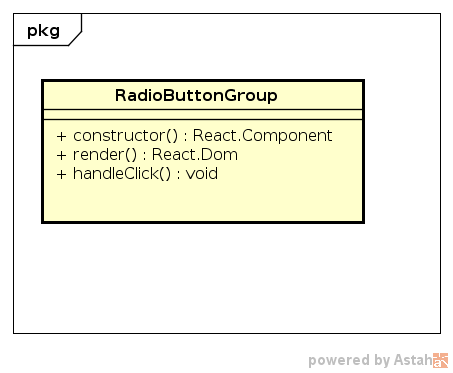
\includegraphics[width=0.6\textwidth]{img/single-RadioButtonGroup}
   \caption{{Diagramma per RadioButtonGroup in UI-SingleComponents}}
\end{figure}
\FloatBarrier
\textbf{Descrizione}\\
Componente React che rappresenta un insieme di radio button tra cui è possibile scegliere tra opzioni mutualmente esclusive.\\\\
\textbf{Metodi:} \begin{itemize}\item +constructor(props : Object) : React.Component \\Costruttore della sottoclasse di React.Component in cui è necessario chiamare super (props) ed è possibile inizializzare lo stato per i dati soggetti a cambiamento.\item +handleChange(): void \\Viene invocato il metodo passato dal genitore\item +render() : React.DOM \\Metodo che esamina this.props e this.state e restituisce un singolo elemento React che può essere una rappresentazione di un componente DOM nativo o un altro componente composito.\end{itemize} 


\textbf{Applicazioni}\\
Viene utilizzato per costruire le interfacce grafiche delle bolle. 


\clearpage

\subsubsection{TextAreaComboBox}
\textbf{Componente:}  Monolith::UI::UI-SingleComponents\\
   \FloatBarrier
   \begin{figure}[ht]
   \centering
   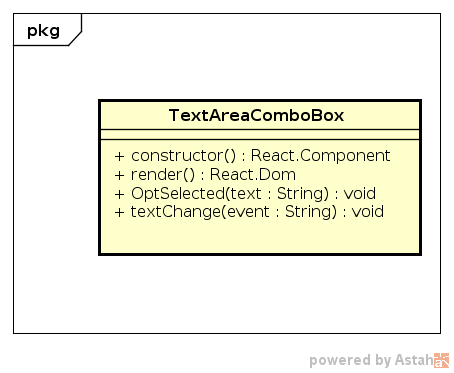
\includegraphics[width=0.6\textwidth]{img/single-TextAreaComboBox}
   \caption{{Diagramma per TextAreaComboBox in UI-SingleComponents}}
\end{figure}
\FloatBarrier
\textbf{Descrizione}\\
Componente React che rappresenta una TextArea con a fianco un ComboBox \\\\
\textbf{Metodi:} \begin{itemize}\item +constructor(props : Object) : React.Component \\Costruttore della sottoclasse di React.Component in cui è necessario chiamare super (props) ed è possibile inizializzare lo stato per i dati soggetti a cambiamento.\item +OptSelected(text : String) : void \\ Comunica l'opzione selezionata tramite il metodo del genitore.\item +textChange(event : String) : void  \\ Comunica il contenuto della textarea tramite il metodo del genitore \item +render() : React.DOM \\Metodo che esamina this.props e this.state e restituisce un singolo elemento React che può essere una rappresentazione di un componente DOM nativo o un altro componente composito.\end{itemize} 


\textbf{Applicazioni}\\
Viene utilizzato per costruire le interfacce grafiche delle bolle. 


\clearpage

\subsubsection{LineEditPushButton}
\textbf{Componente:}  Monolith::UI::UI-SingleComponents\\
   \FloatBarrier
   \begin{figure}[ht]
   \centering
   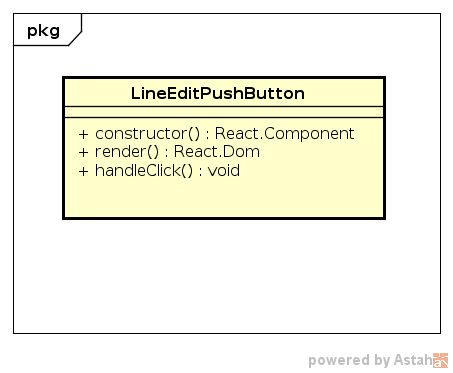
\includegraphics[width=0.6\textwidth]{img/single-LineEditPushButton}
   \caption{{Diagramma per LineEditPushButton in UI-SingleComponents}}
\end{figure}
\FloatBarrier
\textbf{Descrizione}\\
Componente React che rappresenta un campo di inserimento testo affiancato ad un pulsante. \\\\
\textbf{Metodi:} \begin{itemize}\item +constructor(props : Object) : React.Component \\Costruttore della sottoclasse di React.Component in cui è necessario chiamare super (props) ed è possibile inizializzare lo stato per i dati soggetti a cambiamento.\item +handleClick(event : String) : void  \\Viene invocato il metodo passato dal genitore\item +render() : React.DOM \\Metodo che esamina this.props e this.state e restituisce un singolo elemento React che può essere una rappresentazione di un componente DOM nativo o un altro componente composito.\end{itemize} 


\textbf{Applicazioni}\\
Viene utilizzato per costruire le interfacce grafiche delle bolle. 


\clearpage

\subsubsection{LabelEditPushButton}
\textbf{Componente:}  Monolith::UI::UI-SingleComponents\\
   \FloatBarrier
   \begin{figure}[ht]
   \centering
   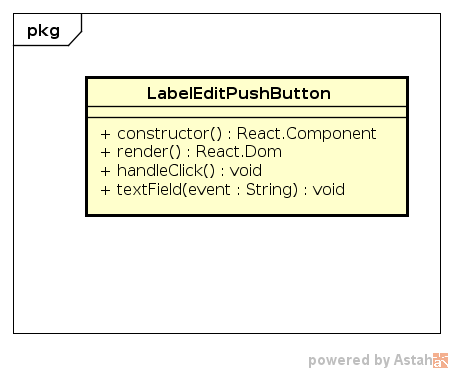
\includegraphics[width=0.6\textwidth]{img/single-LabelEditPushButton}
   \caption{{Diagramma per LabelEditPushButton in UI-SingleComponents}}
\end{figure}
\FloatBarrier
\textbf{Descrizione}\\
Componente React che rappresenta del testo con un pulsante. \\\\
\textbf{Metodi:} \begin{itemize}\item +constructor(props : Object) : React.Component \\Costruttore della sottoclasse di React.Component in cui è necessario chiamare super (props) ed è possibile inizializzare lo stato per i dati soggetti a cambiamento.\item +textField(text : String) : void \\Comunica l’opzione selezionata tramite il metodo del genitore.\item +handleClick(event : String) : void  \\Comunica l’opzione selezionata tramite il metodo del genitore. \item +render() : React.DOM \\Metodo che esamina this.props e this.state e restituisce un singolo elemento React che può essere una rappresentazione di un componente DOM nativo o un altro componente composito.\end{itemize} 


\textbf{Applicazioni}\\
Viene utilizzato per costruire le interfacce grafiche delle bolle. 


\subsection{Architettura di dettaglio - Classi delle bolle demo}\subsubsection{CurrencyConversion}
\textbf{Componente:}  CurrencyBubble\\
   \FloatBarrier
   \begin{figure}[ht]
   \centering
   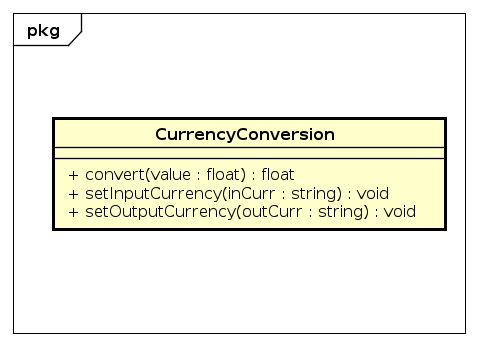
\includegraphics[width=0.6\textwidth]{img/single-CurrencyConversion}
   \caption{{Diagramma per CurrencyConversion in CurrencyBubble}}
\end{figure}
\FloatBarrier
\textbf{Descrizione}\\
Classe predisposta per la conversione di un importo da una valuta di partenza a una valuta di arrivo.
\\
\\
\textbf{Metodi:} 
\begin{itemize}
\item +convert(value : float) : float 
\\
Metodo che effettua la conversione del valore utilizzando l'utility money.js.
\item +setInputCurrency(inCurr : string) : void 
\\
Metodo che imposta la valuta di partenza.
\item +setOutputCurrency(outCurr : string) : void 
\\
Metodo che imposta la valuta di arrivo.
\end{itemize} 


\textbf{Applicazioni}\\
Viene utilizzata per effettuare la conversione di un importo dalla valuta di partenza a quella di arrivo. Si serve dell'utility money.js. 


\clearpage

\subsubsection{CurrencyBubbleSender}
\textbf{Componente:}  CurrencyBubble\\
   \FloatBarrier
   \begin{figure}[ht]
   \centering
   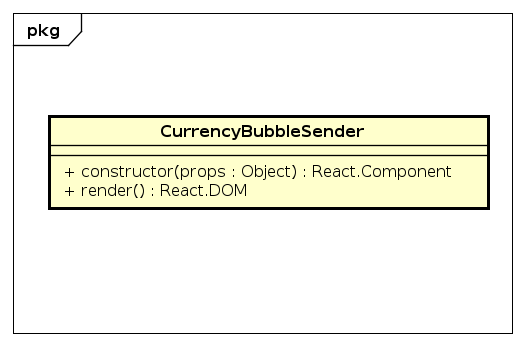
\includegraphics[width=0.6\textwidth]{img/single-CurrencyBubbleSender}
   \caption{{Diagramma per CurrencyBubbleSender in CurrencyBubble}}
\end{figure}
\FloatBarrier
\textbf{Descrizione}\\
Istanziazione concreta della classe Monolith::Bubbles::Bubble che rappresenta la bolla vista dal mittente.
\\
\\
\textbf{Metodi:} 
\begin{itemize}
\item +constructor(props : Object) : React.Component 
\\
Costruttore della sottoclasse di React.Component in cui è necessario chiamare super (props) ed è possibile inizializzare lo stato per i dati soggetti a cambiamento.

\item +render() : React.DOM
Metodo che esamina this.props e this.state e restituisce un singolo elemento React che può essere una rappresentazione di un componente DOM nativo o un altro componente composito.

\end{itemize} 


\textbf{Applicazioni}\\
Viene utilizzata per la visualizzazione della bolla da parte del mittente. 


\clearpage

\subsubsection{CurrencyBubbleCreator}
\textbf{Componente:}  CurrencyBubble\\
   \FloatBarrier
   \begin{figure}[ht]
   \centering
   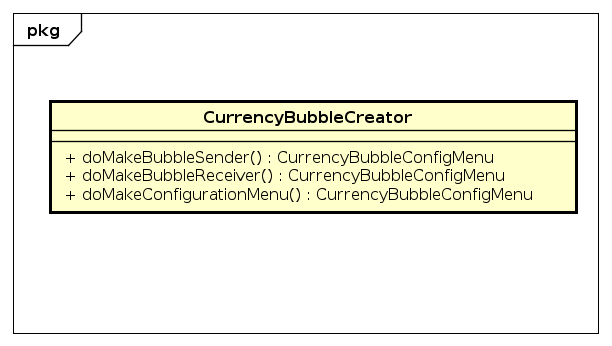
\includegraphics[width=0.6\textwidth]{img/single-CurrencyBubbleCreator}
   \caption{{Diagramma per CurrencyBubbleCreator in CurrencyBubble}}
\end{figure}
\FloatBarrier
\textbf{Descrizione}\\
Istanziazione concreta della classe Monolith::UI::Bubbles::BubbleCreator che gestisce la creazione della singola istanza di bolla convertitore di valuta, della singola istanza di menù di configurazione della bolla e della singola istanza di pulsante tramite l'utilizzo della classe Monolith::UI::Bubbles::BubbleDiscriminator.
\\
\\
\textbf{Metodi:} 
\begin{itemize}
\item +doMakeBubbleSender() : CurrencyBubble 
\\
Metodo che gestisce la creazione della bolla vista dal mittente.
\item +doMakeBubbleReceiver() : CurrencyBubble 
\\
Metodo che gestisce la creazione della bolla vista dal ricevente.
\item +doMakeConfigurationMenu() : CurrencyBubbleConfig 
\\
Metodo che gestisce la creazione dell'area di configurazione della bolla.
\item +doMakeButton() : CurrencyBubbleCreationButton 
\\
Metodo che gestisce la creazione della singola istanza di pulsante da inserire nel menu iniziale di creazione. Viene lasciata l'implementazione della super classe.
\end{itemize} 


\textbf{Applicazioni}\\
Viene utilizzata per gestire la creazione della singola istanza di bolla convertitore di valuta, della singola istanza di menù di configurazione della bolla e della singola istanza di pulsante. 


\clearpage

\subsubsection{CurrencyBubbleReceiver}
\textbf{Componente:}  CurrencyBubble\\
   \FloatBarrier
   \begin{figure}[ht]
   \centering
   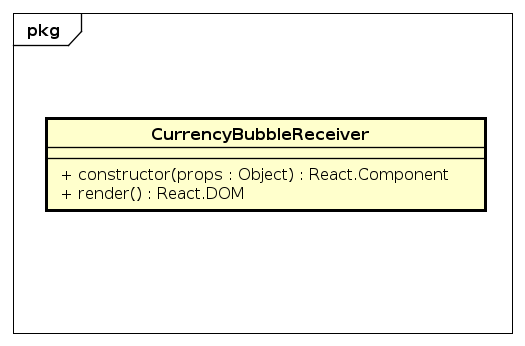
\includegraphics[width=0.6\textwidth]{img/single-CurrencyBubbleReceiver}
   \caption{{Diagramma per CurrencyBubbleReceiver in CurrencyBubble}}
\end{figure}
\FloatBarrier
\textbf{Descrizione}\\
Istanziazione concreta della classe Monolith::Bubbles::Bubble che rappresenta la bolla vista dal ricevente.
\\
\\
\textbf{Metodi:} 
\begin{itemize}
\item +constructor(props : Object) : React.Component 
\\
Costruttore della sottoclasse di React.Component in cui è necessario chiamare super (props) ed è possibile inizializzare lo stato per i dati soggetti a cambiamento.

\item +render() : React.DOM
Metodo che esamina this.props e this.state e restituisce un singolo elemento React che può essere una rappresentazione di un componente DOM nativo o un altro componente composito.

\end{itemize} 


\textbf{Applicazioni}\\
Viene utilizzata per la visualizzazione della bolla da parte del ricevente. 


\clearpage

\subsubsection{CurrencyBubbleConfigMenu}
\textbf{Componente:}  CurrencyBubble\\
   \FloatBarrier
   \begin{figure}[ht]
   \centering
   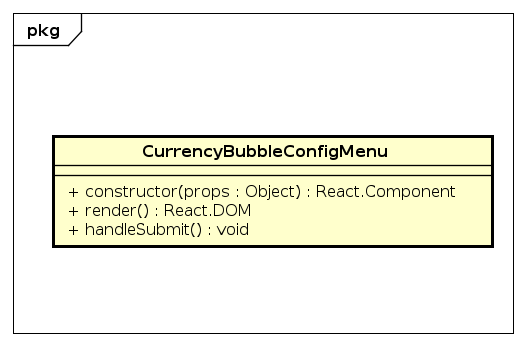
\includegraphics[width=0.6\textwidth]{img/single-CurrencyBubbleConfigMenu}
   \caption{{Diagramma per CurrencyBubbleConfigMenu in CurrencyBubble}}
\end{figure}
\FloatBarrier
\textbf{Descrizione}\\
Istanziazione concreta della classe Monolith::UI::Bubbles::BubbleConfig che rappresenta l'area di configurazione della bolla. 
\\
\\
\textbf{Metodi:} 
\begin{itemize}
\item +constructor(props : Object) : React.Component 
\\
Costruttore della sottoclasse di React.Component in cui è necessario chiamare super (props) ed è possibile inizializzare lo stato per i dati soggetti a cambiamento.

\item +render() : React.DOM
Metodo che esamina this.props e this.state e restituisce un singolo elemento React che può essere una rappresentazione di un componente DOM nativo o un altro componente composito.

\item + handleSubmit() : void
Metodo che viene invocato quando la configurazione della bolla è terminata ed è pronta per essere inviata.

\end{itemize} 


\textbf{Applicazioni}\\
Viene utilizzata per la visualizzazione dell'area di configurazione della bolla. 


\clearpage

\subsubsection{DiceRoller}
\textbf{Componente:}  DiceBubble\\
   \FloatBarrier
   \begin{figure}[ht]
   \centering
   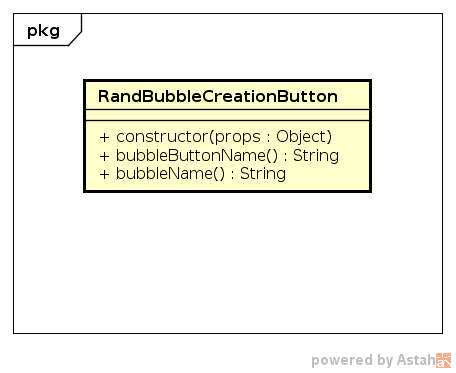
\includegraphics[width=0.6\textwidth]{img/single-DiceRoller}
   \caption{{Diagramma per DiceRoller in DiceBubble}}
\end{figure}
\FloatBarrier
\textbf{Descrizione}\\
Classe predisposta per l'estrazione del numero casuale.
\\
\\
\textbf{Metodi:} 
\begin{itemize}
\item +roll(max : int) : int
Metodo che effettua l'estrazione del numero casuale utilizzando la funzione Javascript Math.random().
\end{itemize} 


\textbf{Applicazioni}\\
Viene utilizzata per l'estrazione del numero casuale compreso tra 0 e max. Si serve della funzione Javascript Math.random(). 


\clearpage

\subsubsection{DiceBubbleSender}
\textbf{Componente:}  DiceBubble\\
   \FloatBarrier
   \begin{figure}[ht]
   \centering
   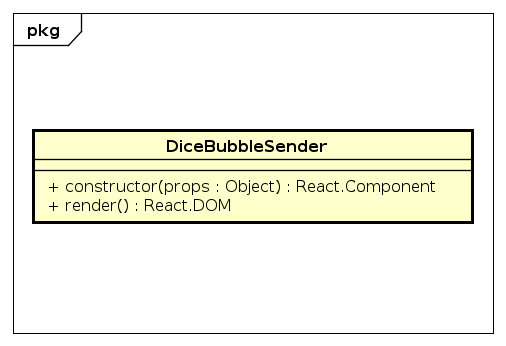
\includegraphics[width=0.6\textwidth]{img/single-DiceBubbleSender}
   \caption{{Diagramma per DiceBubbleSender in DiceBubble}}
\end{figure}
\FloatBarrier
\textbf{Descrizione}\\
Istanziazione concreta della classe Monolith::Bubbles::Bubble che rappresenta la bolla vista dal mittente.
\\
\\
\textbf{Metodi:} 
\begin{itemize}
\item +constructor(props : Object) : React.Component 
\\
Costruttore della sottoclasse di React.Component in cui è necessario chiamare super (props) ed è possibile inizializzare lo stato per i dati soggetti a cambiamento.

\item +render() : React.DOM
Metodo che esamina this.props e this.state e restituisce un singolo elemento React che può essere una rappresentazione di un componente DOM nativo o un altro componente composito.

\end{itemize} 


\textbf{Applicazioni}\\
Viene utilizzata per la visualizzazione della bolla da parte del mittente. 


\clearpage

\subsubsection{DiceBubbleCreator}
\textbf{Componente:}  DiceBubble\\
   \FloatBarrier
   \begin{figure}[ht]
   \centering
   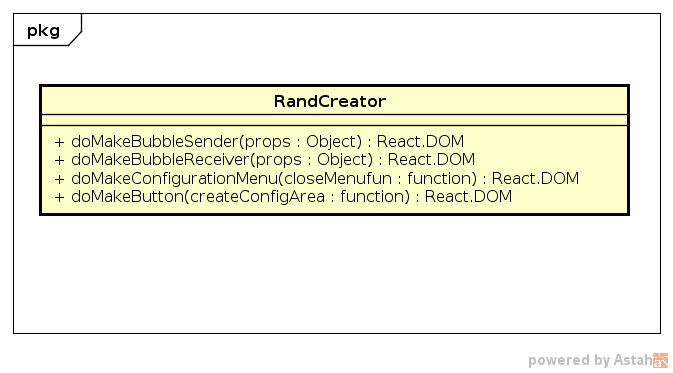
\includegraphics[width=0.6\textwidth]{img/single-DiceBubbleCreator}
   \caption{{Diagramma per DiceBubbleCreator in DiceBubble}}
\end{figure}
\FloatBarrier
\textbf{Descrizione}\\
Istanziazione concreta della classe Monolith::UI::Bubbles::BubbleCreator che gestisce la creazione della singola istanza di bolla estrazione di numero casuale, della singola istanza di menù di configurazione della bolla e della singola istanza di pulsante tramite l'utilizzo della classe Monolith::UI::Bubbles::BubbleDiscriminator.
\\
\\
\textbf{Metodi:} 
\begin{itemize}
\item +doMakeBubbleSender() : DiceBubble 
\\
Metodo che gestisce la creazione della bolla vista dal mittente.
\item +doMakeBubbleReceiver() : DiceBubble 
\\
Metodo che gestisce la creazione della bolla vista dal ricevente.
\item +doMakeConfigurationMenu() : DiceBubbleConfig 
\\
Metodo che gestisce la creazione dell'area di configurazione della bolla.
\item +doMakeButton() : DiceBubbleCreationButton 
\\
Metodo che gestisce la creazione della singola istanza di pulsante da inserire nel menu iniziale di creazione. Viene lasciata l'implementazione della super classe.
\end{itemize} 


\textbf{Applicazioni}\\
Viene utilizzata per gestire la creazione della singola istanza di bolla estrazione di numero casuale, della singola istanza di menù di configurazione della bolla e della singola istanza di pulsante. 


\clearpage

\subsubsection{DiceBubbleReceiver}
\textbf{Componente:}  DiceBubble\\
   \FloatBarrier
   \begin{figure}[ht]
   \centering
   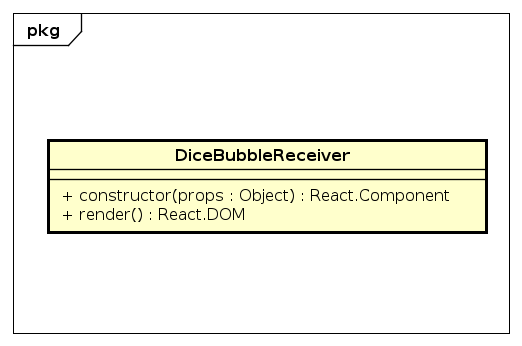
\includegraphics[width=0.6\textwidth]{img/single-DiceBubbleReceiver}
   \caption{{Diagramma per DiceBubbleReceiver in DiceBubble}}
\end{figure}
\FloatBarrier
\textbf{Descrizione}\\
Istanziazione concreta della classe Monolith::Bubbles::Bubble che rappresenta la bolla vista dal ricevente.
\\
\\
\textbf{Metodi:} 
\begin{itemize}
\item +constructor(props : Object) : React.Component 
\\
Costruttore della sottoclasse di React.Component in cui è necessario chiamare super (props) ed è possibile inizializzare lo stato per i dati soggetti a cambiamento.

\item +render() : React.DOM
Metodo che esamina this.props e this.state e restituisce un singolo elemento React che può essere una rappresentazione di un componente DOM nativo o un altro componente composito.

\end{itemize} 


\textbf{Applicazioni}\\
Viene utilizzata per la visualizzazione della bolla da parte del ricevente. 


\clearpage

\subsubsection{DiceBubbleConfigMenu}
\textbf{Componente:}  DiceBubble\\
   \FloatBarrier
   \begin{figure}[ht]
   \centering
   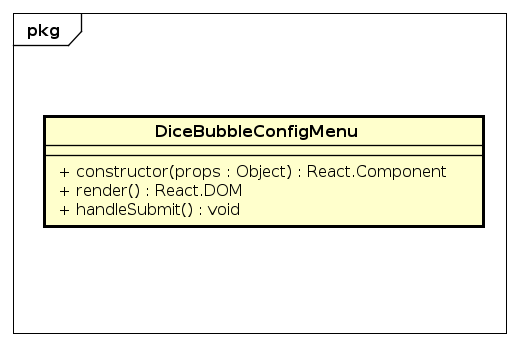
\includegraphics[width=0.6\textwidth]{img/single-DiceBubbleConfigMenu}
   \caption{{Diagramma per DiceBubbleConfigMenu in DiceBubble}}
\end{figure}
\FloatBarrier
\textbf{Descrizione}\\
Istanziazione concreta della classe Monolith::UI::Bubbles::BubbleConfig che rappresenta l'area di configurazione della bolla. 
\\
\\
\textbf{Metodi:} 
\begin{itemize}
\item +constructor(props : Object) : React.Component 
\\
Costruttore della sottoclasse di React.Component in cui è necessario chiamare super (props) ed è possibile inizializzare lo stato per i dati soggetti a cambiamento.

\item +render() : React.DOM
Metodo che esamina this.props e this.state e restituisce un singolo elemento React che può essere una rappresentazione di un componente DOM nativo o un altro componente composito.

\item +handleSubmit() : void
Metodo che viene invocato quando la configurazione della bolla è terminata ed è pronta per essere inviata.

\end{itemize} 


\textbf{Applicazioni}\\
Viene utilizzata per la visualizzazione dell'area di configurazione della bolla. 


\clearpage

\subsubsection{CheckListCreator}
\textbf{Componente:}  ListBubble::CheckListCreation\\
   \FloatBarrier
   \begin{figure}[ht]
   \centering
   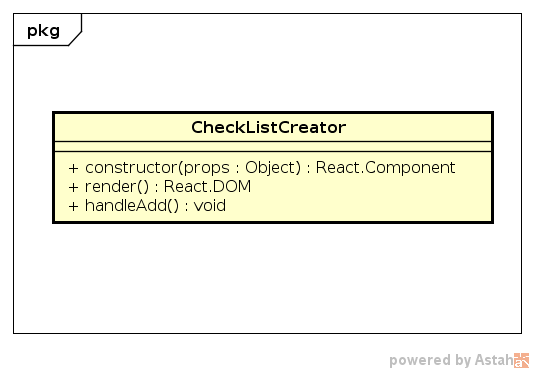
\includegraphics[width=0.6\textwidth]{img/single-CheckListCreator}
   \caption{{Diagramma per CheckListCreator in CheckListCreation}}
\end{figure}
\FloatBarrier
\textbf{Descrizione}\\
Componente React che rappresenta l'area di visualizzazione delle check list e un pulsante per poterne aggiungere di nuove. 
\\
\\
\textbf{Metodi:} 
\begin{itemize}
\item +constructor(props : Object) : React.Component 
\\
Costruttore della sottoclasse di React.Component in cui è necessario chiamare super (props) ed è possibile inizializzare lo stato per i dati soggetti a cambiamento.

\item +render() : React.DOM
Metodo che esamina this.props e this.state e restituisce un singolo elemento React che può essere una rappresentazione di un componente DOM nativo o un altro componente composito.

\item +handleAdd() : void
Metodo che gestisce l'aggiunta di una nuova check list. 
\end{itemize} 


\textbf{Applicazioni}\\
Viene utilizzato per rappresentare l'area di visualizzazione delle check list e un pulsante per poterne aggiungere di nuove. 


\clearpage

\subsubsection{CheckListComponent}
\textbf{Componente:}  ListBubble::CheckListCreation\\
   \FloatBarrier
   \begin{figure}[ht]
   \centering
   \includegraphics[width=0.6\textwidth]{img/single-CheckListComponent}
   \caption{{Diagramma per CheckListComponent in CheckListCreation}}
\end{figure}
\FloatBarrier
\textbf{Descrizione}\\
Componente React che rappresenta una lista di check list.
\\
\\
\textbf{Metodi:} 
\begin{itemize}
\item +constructor(props : Object) : React.Component 
\\
Costruttore della sottoclasse di React.Component in cui è necessario chiamare super (props) ed è possibile inizializzare lo stato per i dati soggetti a cambiamento.

\item +render() : React.DOM
Metodo che esamina this.props e this.state e restituisce un singolo elemento React che può essere una rappresentazione di un componente DOM nativo o un altro componente composito.

\end{itemize} 


\textbf{Applicazioni}\\
Viene utilizzato per rappresentare una lista di check list. 


\clearpage

\subsubsection{CheckListItemsDefinition}
\textbf{Componente:}  ListBubble::CheckListCreation\\
   \FloatBarrier
   \begin{figure}[ht]
   \centering
   \includegraphics[width=0.6\textwidth]{img/single-CheckListItemsDefinition}
   \caption{{Diagramma per CheckListItemsDefinition in CheckListCreation}}
\end{figure}
\FloatBarrier
\textbf{Descrizione}\\
Componente React che rappresenta l'area di configurazione di una check list.
\\
\\
\textbf{Metodi:} 
\begin{itemize}
\item +constructor(props : Object) : React.Component 
\\
Costruttore della sottoclasse di React.Component in cui è necessario chiamare super (props) ed è possibile inizializzare lo stato per i dati soggetti a cambiamento.

\item +render() : React.DOM
Metodo che esamina this.props e this.state e restituisce un singolo elemento React che può essere una rappresentazione di un componente DOM nativo o un altro componente composito.

\end{itemize} 


\textbf{Applicazioni}\\
Viene utilizzato per rappresentare l'area di configurazione di una check list. 


\clearpage

\subsubsection{CheckList}
\textbf{Componente:}  ListBubble::CheckListReading\\
   \FloatBarrier
   \begin{figure}[ht]
   \centering
   \includegraphics[width=0.6\textwidth]{img/single-CheckList}
   \caption{{Diagramma per CheckList in CheckListReading}}
\end{figure}
\FloatBarrier
\textbf{Descrizione}\\
Componente React che gestisce l'aggiunta di un elemento alla lista.
\\
\\
\textbf{Metodi:} 
\begin{itemize}
\item +constructor(props : Object) : React.Component 
\\
Costruttore della sottoclasse di React.Component in cui è necessario chiamare super (props) ed è possibile inizializzare lo stato per i dati soggetti a cambiamento.

\item +render() : React.DOM 
\\
Metodo che esamina this.props e this.state e restituisce un singolo elemento React che può essere una rappresentazione di un componente DOM nativo o un altro componente composito.

\item +handleAdd() : void 
\\
Metodo che gestisce l'aggiunta di un elemento alla lista.
\end{itemize} 


\textbf{Applicazioni}\\
Viene utilizzata per gestire l'aggiunta di un elemento alla lista. 


\clearpage

\subsubsection{ListOfCheckLists}
\textbf{Componente:}  ListBubble::CheckListReading\\
   \FloatBarrier
   \begin{figure}[ht]
   \centering
   \includegraphics[width=0.6\textwidth]{img/single-ListOfCheckLists}
   \caption{{Diagramma per ListOfCheckLists in CheckListReading}}
\end{figure}
\FloatBarrier
\textbf{Descrizione}\\
Componente React che rappresenta una lista di check list.
\\
\\
\textbf{Metodi:} 
\begin{itemize}
\item +constructor(props : Object) : React.Component 
\\
Costruttore della sottoclasse di React.Component in cui è necessario chiamare super (props) ed è possibile inizializzare lo stato per i dati soggetti a cambiamento.

\item +render() : React.DOM
Metodo che esamina this.props e this.state e restituisce un singolo elemento React che può essere una rappresentazione di un componente DOM nativo o un altro componente composito.

\end{itemize} 


\textbf{Applicazioni}\\
Viene utilizzata per la visualizzazione della lista di check list. 


\clearpage

\subsubsection{ListCreationButton}
\textbf{Componente:}  ListBubble::Configuration\\
   \FloatBarrier
   \begin{figure}[ht]
   \centering
   \includegraphics[width=0.6\textwidth]{img/single-ListCreationButton}
   \caption{{Diagramma per ListCreationButton in Configuration}}
\end{figure}
\FloatBarrier
\textbf{Descrizione}\\
Istanziazione della classe Monolith::UI::Bubbles::BubbleCreationButton che rappresenta la singola istanza di pulsante da inserire nel menu iniziale di creazione.
\\
\\
\textbf{Metodi:} 
\begin{itemize}
\item +constructor(props : Object) : React.Component 
\\
Costruttore della sottoclasse di React.Component in cui è necessario chiamare super (props) ed è possibile inizializzare lo stato per i dati soggetti a cambiamento.

\item +render() : React.DOM
Metodo che esamina this.props e this.state e restituisce un singolo elemento React che può essere una rappresentazione di un componente DOM nativo o un altro componente composito.

\end{itemize} 


\textbf{Applicazioni}\\
Viene utilizzata per rappresentare la singola istanza di pulsante da inserire nel menu iniziale di creazione. 


\clearpage

\subsubsection{ListBubbleMenuConfig}
\textbf{Componente:}  ListBubble::Configuration\\
   \FloatBarrier
   \begin{figure}[ht]
   \centering
   \includegraphics[width=0.6\textwidth]{img/single-ListBubbleMenuConfig}
   \caption{{Diagramma per ListBubbleMenuConfig in Configuration}}
\end{figure}
\FloatBarrier
\textbf{Descrizione}\\
Istanziazione concreta della classe Monolith::UI::Bubbles::BubbleConfig che rappresenta l'area di configurazione della bolla. 
\\
\\
\textbf{Metodi:} 
\begin{itemize}
\item +constructor(props : Object) : React.Component 
\\
Costruttore della sottoclasse di React.Component in cui è necessario chiamare super (props) ed è possibile inizializzare lo stato per i dati soggetti a cambiamento.

\item +render() : React.DOM 
\\
Metodo che esamina this.props e this.state e restituisce un singolo elemento React che può essere una rappresentazione di un componente DOM nativo o un altro componente composito.

\item +handleSubmit() : void 
\\
Metodo che viene invocato quando la configurazione della bolla è terminata ed è pronta per essere inviata.

\item +handleAdd() : void 
\\
Metodo che viene invocato quando si vuole aggiungere un elemento alla lista.
\end{itemize} 


\textbf{Applicazioni}\\
Viene utilizzata per la visualizzazione dell'area di configurazione della bolla. 


\clearpage

\subsubsection{ListBubbleCreator}
\textbf{Componente:}  ListBubble::DataManagement\\
   \FloatBarrier
   \begin{figure}[ht]
   \centering
   \includegraphics[width=0.6\textwidth]{img/single-ListBubbleCreator}
   \caption{{Diagramma per ListBubbleCreator in DataManagement}}
\end{figure}
\FloatBarrier
\textbf{Descrizione}\\
Istanziazione concreta della classe Monolith::UI::Bubbles::BubbleCreator che gestisce la creazione della singola istanza di bolla lista, della singola istanza di menù di configurazione della bolla e della singola istanza di pulsante tramite l'utilizzo della classe Monolith::UI::Bubbles::BubbleDiscriminator.
\\
\\
\textbf{Metodi:} 
\begin{itemize}
\item +doMakeBubbleSender() : ListBubble 
\\
Metodo che gestisce la creazione della bolla vista dal mittente.
\item +doMakeBubbleReceiver() : ListBubble 
\\
Metodo che gestisce la creazione della bolla vista dal ricevente.
\item +doMakeConfigurationMenu() : ListBubbleConfig 
\\
Metodo che gestisce la creazione dell'area di configurazione della bolla.
\item +doMakeButton() : ListBubbleCreationButton 
\\
Metodo che gestisce la creazione dello specifico pulsante da inserire nel menu iniziale di creazione.
\end{itemize} 


\textbf{Applicazioni}\\
Viene utilizzata per gestire la creazione della singola istanza di bolla lista, della singola istanza di menù di configurazione della bolla e della singola istanza di pulsante. 


\clearpage

\subsubsection{ListBubbleReceiver}
\textbf{Componente:}  ListBubble::Receiver\\
   \FloatBarrier
   \begin{figure}[ht]
   \centering
   \includegraphics[width=0.6\textwidth]{img/single-ListBubbleReceiver}
   \caption{{Diagramma per ListBubbleReceiver in Receiver}}
\end{figure}
\FloatBarrier
\textbf{Descrizione}\\
Istanziazione concreta della classe Monolith::Bubbles::Bubble che rappresenta la bolla vista dal ricevente.
\\
\\
\textbf{Metodi:} 
\begin{itemize}
\item +constructor(props : Object) : React.Component 
\\
Costruttore della sottoclasse di React.Component in cui è necessario chiamare super (props) ed è possibile inizializzare lo stato per i dati soggetti a cambiamento.

\item +render() : React.DOM 
\\
Metodo che esamina this.props e this.state e restituisce un singolo elemento React che può essere una rappresentazione di un componente DOM nativo o un altro componente composito.

\item +handleCheck() : void 
\\
Metodo che gestisce la spunta di un elemento della lista.
\end{itemize} 


\textbf{Applicazioni}\\
Viene utilizzata per la visualizzazione della bolla da parte del ricevente. 


\clearpage

\subsubsection{ListBubbleSender}
\textbf{Componente:}  ListBubble::Sender\\
   \FloatBarrier
   \begin{figure}[ht]
   \centering
   \includegraphics[width=0.6\textwidth]{img/single-ListBubbleSender}
   \caption{{Diagramma per ListBubbleSender in Sender}}
\end{figure}
\FloatBarrier
\textbf{Descrizione}\\
Istanziazione concreta della classe Monolith::Bubbles::Bubble che rappresenta la bolla vista dal mittente.
\\
\\
\textbf{Metodi:} 
\begin{itemize}
\item +constructor(props : Object) : React.Component 
\\
Costruttore della sottoclasse di React.Component in cui è necessario chiamare super (props) ed è possibile inizializzare lo stato per i dati soggetti a cambiamento.

\item +render() : React.DOM 
\\
Metodo che esamina this.props e this.state e restituisce un singolo elemento React che può essere una rappresentazione di un componente DOM nativo o un altro componente composito.

\item +handleAdd() : void 
\\
Metodo che gestisce l'aggiunta di un nuovo elemento alla lista.
\item +handleCheck() : void 
\\
Metodo che gestisce la spunta di un elemento della lista.
\end{itemize} 


\textbf{Applicazioni}\\
Viene utilizzata per la visualizzazione della bolla da parte del mittente. 


\clearpage

\subsubsection{MeteoItem}
\textbf{Componente:}  MeteoBubble\\
   \FloatBarrier
   \begin{figure}[ht]
   \centering
   \includegraphics[width=0.6\textwidth]{img/single-MeteoItem}
   \caption{{Diagramma per MeteoItem in MeteoBubble}}
\end{figure}
\FloatBarrier
\textbf{Descrizione}\\
Componente React predisposto per la visualizzazione delle previsioni meteo.
\\
\\
\textbf{Metodi:} 
\begin{itemize}
\item +constructor(props : Object) : React.Component 
\\
Costruttore della sottoclasse di React.Component in cui è necessario chiamare super (props) ed è possibile inizializzare lo stato per i dati soggetti a cambiamento.

\item +render() : React.DOM
Metodo che esamina this.props e this.state e restituisce un singolo elemento React che può essere una rappresentazione di un componente DOM nativo o un altro componente composito.

\end{itemize} 


\textbf{Applicazioni}\\
Viene utilizzata per la visualizzazione delle previsioni meteo di un determinato giorno. 


\clearpage

\subsubsection{MeteoDelivery}
\textbf{Componente:}  MeteoBubble\\
   \FloatBarrier
   \begin{figure}[ht]
   \centering
   \includegraphics[width=0.6\textwidth]{img/single-MeteoDelivery}
   \caption{{Diagramma per MeteoDelivery in MeteoBubble}}
\end{figure}
\FloatBarrier
\textbf{Descrizione}\\
Classe predisposta per il recupero dei dati relativi alle previsioni meteo.
\\
\\
\textbf{Metodi:} 
\begin{itemize}
\item +getData(location : string) : Object
Metodo che recupera i dati relativi alle previsioni meteo della località selezionata utilizzando l'utility weather.js.

\end{itemize} 


\textbf{Applicazioni}\\
Viene utilizzata per recuperare i dati relativi alle previsioni meteo della località scelta. Si serve dell'utility weather.js. 


\clearpage

\subsubsection{MeteoBubbleSender}
\textbf{Componente:}  MeteoBubble\\
   \FloatBarrier
   \begin{figure}[ht]
   \centering
   \includegraphics[width=0.6\textwidth]{img/single-MeteoBubbleSender}
   \caption{{Diagramma per MeteoBubbleSender in MeteoBubble}}
\end{figure}
\FloatBarrier
\textbf{Descrizione}\\
Istanziazione concreta della classe Monolith::Bubbles::Bubble che rappresenta la bolla vista dal mittente.
\\
\\
\textbf{Metodi:} 
\begin{itemize}
\item +constructor(props : Object) : React.Component 
\\
Costruttore della sottoclasse di React.Component in cui è necessario chiamare super (props) ed è possibile inizializzare lo stato per i dati soggetti a cambiamento.

\item +render() : React.DOM
Metodo che esamina this.props e this.state e restituisce un singolo elemento React che può essere una rappresentazione di un componente DOM nativo o un altro componente composito.

\end{itemize} 


\textbf{Applicazioni}\\
Viene utilizzata per la visualizzazione della bolla da parte del mittente. 


\clearpage

\subsubsection{MeteoBubbleCreator}
\textbf{Componente:}  MeteoBubble\\
   \FloatBarrier
   \begin{figure}[ht]
   \centering
   \includegraphics[width=0.6\textwidth]{img/single-MeteoBubbleCreator}
   \caption{{Diagramma per MeteoBubbleCreator in MeteoBubble}}
\end{figure}
\FloatBarrier
\textbf{Descrizione}\\
Istanziazione concreta della classe Monolith::UI::Bubbles::BubbleCreator che gestisce la creazione della singola istanza di bolla meteo, della singola istanza di menù di configurazione della bolla e della singola istanza di pulsante tramite l'utilizzo della classe Monolith::UI::Bubbles::BubbleDiscriminator.
\\
\\
\textbf{Metodi:} 
\begin{itemize}
\item +doMakeBubbleSender() : MeteoBubble 
\\
Metodo che gestisce la creazione della bolla vista dal mittente.
\item +doMakeBubbleReceiver() : MeteoBubble 
\\
Metodo che gestisce la creazione della bolla vista dal ricevente.
\item +doMakeConfigurationMenu() : MeteoBubbleConfig 
\\
Metodo che gestisce la creazione dell'area di configurazione della bolla.
\item +doMakeButton() : MeteoBubbleCreationButton 
\\
Metodo che gestisce la creazione dello specifico pulsante da inserire nel menu iniziale di creazione. Viene lasciata l'implementazione della super classe.
\end{itemize} 


\textbf{Applicazioni}\\
Viene utilizzata per gestire la creazione della singola istanza di bolla meteo, della singola istanza di menù di configurazione della bolla e della singola istanza di pulsante. 


\clearpage

\subsubsection{MeteoBubbleReceiver}
\textbf{Componente:}  MeteoBubble\\
   \FloatBarrier
   \begin{figure}[ht]
   \centering
   \includegraphics[width=0.6\textwidth]{img/single-MeteoBubbleReceiver}
   \caption{{Diagramma per MeteoBubbleReceiver in MeteoBubble}}
\end{figure}
\FloatBarrier
\textbf{Descrizione}\\
Istanziazione concreta della classe Monolith::Bubbles::Bubble che rappresenta la bolla vista dal ricevente.
\\
\\
\textbf{Metodi:} 
\begin{itemize}
\item +constructor(props : Object) : React.Component 
\\
Costruttore della sottoclasse di React.Component in cui è necessario chiamare super (props) ed è possibile inizializzare lo stato per i dati soggetti a cambiamento.

\item +render() : React.DOM
Metodo che esamina this.props e this.state e restituisce un singolo elemento React che può essere una rappresentazione di un componente DOM nativo o un altro componente composito.

\end{itemize} 


\textbf{Applicazioni}\\
Viene utilizzata per la visualizzazione della bolla da parte del ricevente. 


\clearpage

\subsubsection{MeteoBubbleConfigMenu}
\textbf{Componente:}  MeteoBubble\\
   \FloatBarrier
   \begin{figure}[ht]
   \centering
   \includegraphics[width=0.6\textwidth]{img/single-MeteoBubbleConfigMenu}
   \caption{{Diagramma per MeteoBubbleConfigMenu in MeteoBubble}}
\end{figure}
\FloatBarrier
\textbf{Descrizione}\\
Istanziazione concreta della classe Monolith::UI::Bubbles::BubbleConfig che rappresenta l'area di configurazione della bolla. 
\\
\\
\textbf{Metodi:} 
\begin{itemize}
\item +constructor(props : Object) : React.Component 
\\
Costruttore della sottoclasse di React.Component in cui è necessario chiamare super (props) ed è possibile inizializzare lo stato per i dati soggetti a cambiamento.

\item +render() : React.DOM
Metodo che esamina this.props e this.state e restituisce un singolo elemento React che può essere una rappresentazione di un componente DOM nativo o un altro componente composito.

\item +handleSubmit() : void
Metodo che viene invocato quando la configurazione della bolla è terminata ed è pronta per essere inviata.

\end{itemize} 


\textbf{Applicazioni}\\
Viene utilizzata per la visualizzazione dell'area di configurazione della bolla. 


\clearpage

\subsubsection{ResultsViewer}
\textbf{Componente:}  SurveyBubble\\
   \FloatBarrier
   \begin{figure}[ht]
   \centering
   \includegraphics[width=0.6\textwidth]{img/single-ResultsViewer}
   \caption{{Diagramma per ResultsViewer in SurveyBubble}}
\end{figure}
\FloatBarrier
\textbf{Descrizione}\\
Componente React che rappresenta il risultato del sondaggio.
\\
\\
\textbf{Metodi:} 
\begin{itemize}
\item +constructor(props : Object) : React.Component 
\\
Costruttore della sottoclasse di React.Component in cui è necessario chiamare super (props) ed è possibile inizializzare lo stato per i dati soggetti a cambiamento.

\item +render() : React.DOM
Metodo che esamina this.props e this.state e restituisce un singolo elemento React che può essere una rappresentazione di un componente DOM nativo o un altro componente composito.

\end{itemize} 


\textbf{Applicazioni}\\
Viene utilizzato per la visualizzazione del risultato del sondaggio. 


\clearpage

\subsubsection{SurveyManager}
\textbf{Componente:}  SurveyBubble\\
   \FloatBarrier
   \begin{figure}[ht]
   \centering
   \includegraphics[width=0.6\textwidth]{img/single-SurveyManager}
   \caption{{Diagramma per SurveyManager in SurveyBubble}}
\end{figure}
\FloatBarrier
\textbf{Descrizione}\\
Classe predisposta per la gestione del sondaggio.
\\
\\
\textbf{Metodi:} 
\begin{itemize}
\item +constructor(props : Object) : React.Component 
\\
Costruttore della sottoclasse di React.Component in cui è necessario chiamare super (props) ed è possibile inizializzare lo stato per i dati soggetti a cambiamento.

\item +render() : React.DOM
Metodo che esamina this.props e this.state e restituisce un singolo elemento React che può essere una rappresentazione di un componente DOM nativo o un altro componente composito.

\item +databaseUpdate(item : int) : void
Metodo che gestisce l'aggiornamento del database al cambiare dei voti nel sondaggio.
\end{itemize} 


\textbf{Applicazioni}\\
Viene utilizzata per gestire l'aggiornamento del database al cambiare dei voti nel sondaggio. 


\clearpage

\subsubsection{SurveyBubbleSender}
\textbf{Componente:}  SurveyBubble\\
   \FloatBarrier
   \begin{figure}[ht]
   \centering
   \includegraphics[width=0.6\textwidth]{img/single-SurveyBubbleSender}
   \caption{{Diagramma per SurveyBubbleSender in SurveyBubble}}
\end{figure}
\FloatBarrier
\textbf{Descrizione}\\
Istanziazione concreta della classe Monolith::Bubbles::Bubble che rappresenta la bolla vista dal mittente.
\\
\\
\textbf{Metodi:} 
\begin{itemize}
\item +constructor(props : Object) : React.Component 
\\
Costruttore della sottoclasse di React.Component in cui è necessario chiamare super (props) ed è possibile inizializzare lo stato per i dati soggetti a cambiamento.

\item +render() : React.DOM
Metodo che esamina this.props e this.state e restituisce un singolo elemento React che può essere una rappresentazione di un componente DOM nativo o un altro componente composito.

\item +handleVote() : void
Metodo che viene invocato quando è stata selezionata un'opzione. 

\end{itemize} 


\textbf{Applicazioni}\\
Viene utilizzata per la visualizzazione della bolla da parte del mittente. 


\clearpage

\subsubsection{SurveyBubbleCreator}
\textbf{Componente:}  SurveyBubble\\
   \FloatBarrier
   \begin{figure}[ht]
   \centering
   \includegraphics[width=0.6\textwidth]{img/single-SurveyBubbleCreator}
   \caption{{Diagramma per SurveyBubbleCreator in SurveyBubble}}
\end{figure}
\FloatBarrier
\textbf{Descrizione}\\
Istanziazione concreta della classe Monolith::UI::Bubbles::BubbleCreator che gestisce la creazione della singola istanza di bolla sondaggio, della singola istanza di menù di configurazione della bolla e della singola istanza di pulsante tramite l'utilizzo della classe Monolith::UI::Bubbles::BubbleDiscriminator.
\\
\\
\textbf{Metodi:} 
\begin{itemize}
\item +doMakeBubbleSender() : SurveyBubble 
\\
Metodo che gestisce la creazione della bolla vista dal mittente.
\item +doMakeBubbleReceiver() : SurveyBubble 
\\
Metodo che gestisce la creazione della bolla vista dal ricevente.
\item +doMakeConfigurationMenu() : SurveyBubbleConfig 
\\
Metodo che gestisce la creazione dell'area di configurazione della bolla.
\item +doMakeButton() : SurveyBubbleCreationButton 
\\
Metodo che gestisce la creazione della singola istanza di pulsante da inserire nel menu iniziale di creazione. Viene lasciata l'implementazione della super classe.
\end{itemize} 


\textbf{Applicazioni}\\
Viene utilizzata per gestire la creazione della singola istanza di bolla sondaggio, della singola istanza di menù di configurazione della bolla e della singola istanza di pulsante. 


\clearpage

\subsubsection{SurveyBubbleReceiver}
\textbf{Componente:}  SurveyBubble\\
   \FloatBarrier
   \begin{figure}[ht]
   \centering
   \includegraphics[width=0.6\textwidth]{img/single-SurveyBubbleReceiver}
   \caption{{Diagramma per SurveyBubbleReceiver in SurveyBubble}}
\end{figure}
\FloatBarrier
\textbf{Descrizione}\\
Istanziazione concreta della classe Monolith::Bubbles::Bubble che rappresenta la bolla vista dal ricevente.
\\
\\
\textbf{Metodi:} 
\begin{itemize}
\item +constructor(props : Object) : React.Component 
\\
Costruttore della sottoclasse di React.Component in cui è necessario chiamare super (props) ed è possibile inizializzare lo stato per i dati soggetti a cambiamento.

\item +render() : React.DOM
Metodo che esamina this.props e this.state e restituisce un singolo elemento React che può essere una rappresentazione di un componente DOM nativo o un altro componente composito.

\item +handleVote() : void
Metodo che viene invocato quando è stata selezionata un'opzione. 

\end{itemize} 


\textbf{Applicazioni}\\
Viene utilizzata per la visualizzazione della bolla da parte del ricevente. 


\clearpage

\subsubsection{SurveyBubbleConfigMenu}
\textbf{Componente:}  SurveyBubble\\
   \FloatBarrier
   \begin{figure}[ht]
   \centering
   \includegraphics[width=0.6\textwidth]{img/single-SurveyBubbleConfigMenu}
   \caption{{Diagramma per SurveyBubbleConfigMenu in SurveyBubble}}
\end{figure}
\FloatBarrier
\textbf{Descrizione}\\
Istanziazione concreta della classe Monolith::UI::Bubbles::BubbleConfig che rappresenta l'area di configurazione della bolla. 
\\
\\
\textbf{Metodi:} 
\begin{itemize}
\item +constructor(props : Object) : React.Component 
\\
Costruttore della sottoclasse di React.Component in cui è necessario chiamare super (props) ed è possibile inizializzare lo stato per i dati soggetti a cambiamento.

\item +render() : React.DOM
Metodo che esamina this.props e this.state e restituisce un singolo elemento React che può essere una rappresentazione di un componente DOM nativo o un altro componente composito.

\item +handleSubmit() : void
Metodo che viene invocato quando la configurazione della bolla è terminata ed è pronta per essere inviata.

\end{itemize} 


\textbf{Applicazioni}\\
Viene utilizzata per la visualizzazione dell'area di configurazione della bolla. 


\clearpage

\subsubsection{MessageTranslation}
\textbf{Componente:}  TranslationBubble\\
   \FloatBarrier
   \begin{figure}[ht]
   \centering
   \includegraphics[width=0.6\textwidth]{img/single-MessageTranslation}
   \caption{{Diagramma per MessageTranslation in TranslationBubble}}
\end{figure}
\FloatBarrier
\textbf{Descrizione}\\
Classe predisposta per l'effettiva traduzione del messaggio.
\\
\\
\textbf{Metodi:} 
\begin{itemize}
\item +translate(msg : string) : string 
\\
Metodo che effettua la traduzione del messaggio utilizzando l'utility Polygloth.js.
\item +setInputLanguage(inLang : string) : void 
\\
Metodo che imposta la lingua di partenza.
\item +setOutputlanguage(outLang : string) : void 
\\
Metodo che imposta la lingua di arrivo.
\end{itemize} 


\textbf{Applicazioni}\\
Viene utilizzata per effettuare la traduzione del messaggio di testo dalla lingua di partenza a quella di arrivo. Si serve dell'utility Polygloth.js. 


\clearpage

\subsubsection{TranslationBubbleSender}
\textbf{Componente:}  TranslationBubble\\
   \FloatBarrier
   \begin{figure}[ht]
   \centering
   \includegraphics[width=0.6\textwidth]{img/single-TranslationBubbleSender}
   \caption{{Diagramma per TranslationBubbleSender in TranslationBubble}}
\end{figure}
\FloatBarrier
\textbf{Descrizione}\\
Istanziazione concreta della classe Monolith::Bubbles::Bubble che rappresenta la bolla vista dal mittente.
\\
\\
\textbf{Metodi:} 
\begin{itemize}
\item +constructor(props : Object) : React.Component 
\\
Costruttore della sottoclasse di React.Component in cui è necessario chiamare super (props) ed è possibile inizializzare lo stato per i dati soggetti a cambiamento.

\item +render() : React.DOM
Metodo che esamina this.props e this.state e restituisce un singolo elemento React che può essere una rappresentazione di un componente DOM nativo o un altro componente composito.

\end{itemize} 


\textbf{Applicazioni}\\
Viene utilizzato per la visualizzazione della bolla da parte del mittente. 


\clearpage

\subsubsection{TranslationBubbleCreator}
\textbf{Componente:}  TranslationBubble\\
   \FloatBarrier
   \begin{figure}[ht]
   \centering
   \includegraphics[width=0.6\textwidth]{img/single-TranslationBubbleCreator}
   \caption{{Diagramma per TranslationBubbleCreator in TranslationBubble}}
\end{figure}
\FloatBarrier
\textbf{Descrizione}\\
Istanziazione concreta della classe Monolith::UI::Bubbles::BubbleCreator che gestisce la creazione della singola istanza di bolla traduttore, della singola istanza di menù di configurazione della bolla e della singola istanza di pulsante tramite l'utilizzo della classe Monolith::UI::Bubbles::BubbleDiscriminator.
\\
\\
\textbf{Metodi:} 
\begin{itemize}
\item +doMakeBubbleSender() : TranslationBubble 
\\
Metodo che gestisce la creazione della bolla vista dal mittente.
\item +doMakeBubbleReceiver() : TranslationBubble 
\\
Metodo che gestisce la creazione della bolla vista dal ricevente.
\item +doMakeConfigurationMenu() : TranslationBubbleConfig 
\\
Metodo che gestisce la creazione dell'area di configurazione della bolla.
\item +doMakeButton() : TranslationBubbleCreationButton 
\\
Metodo che gestisce la creazione della singola istanza di pulsante da inserire nel menu iniziale di creazione. Viene lasciata l'implementazione della super classe.
\end{itemize} 


\textbf{Applicazioni}\\
Viene utilizzata per gestire la creazione della singola istanza di bolla traduttore, della singola istanza di menù di configurazione della bolla e della singola istanza di pulsante. 


\clearpage

\subsubsection{TranslationBubbleReceiver}
\textbf{Componente:}  TranslationBubble\\
   \FloatBarrier
   \begin{figure}[ht]
   \centering
   \includegraphics[width=0.6\textwidth]{img/single-TranslationBubbleReceiver}
   \caption{{Diagramma per TranslationBubbleReceiver in TranslationBubble}}
\end{figure}
\FloatBarrier
\textbf{Descrizione}\\
Istanziazione concreta della classe Monolith::Bubbles::Bubble che rappresenta la bolla vista dal ricevente.
\\
\\
\textbf{Metodi:} 
\begin{itemize}
\item +constructor(props : Object) : React.Component 
\\
Costruttore della sottoclasse di React.Component in cui è necessario chiamare super (props) ed è possibile inizializzare lo stato per i dati soggetti a cambiamento.

\item +render() : React.DOM
Metodo che esamina this.props e this.state e restituisce un singolo elemento React che può essere una rappresentazione di un componente DOM nativo o un altro componente composito.

\end{itemize} 


\textbf{Applicazioni}\\
Viene utilizzata per la visualizzazione della bolla da parte del ricevente. 


\clearpage

\subsubsection{TranslationBubbleConfigMenu}
\textbf{Componente:}  TranslationBubble\\
   \FloatBarrier
   \begin{figure}[ht]
   \centering
   \includegraphics[width=0.6\textwidth]{img/single-TranslationBubbleConfigMenu}
   \caption{{Diagramma per TranslationBubbleConfigMenu in TranslationBubble}}
\end{figure}
\FloatBarrier
\textbf{Descrizione}\\
Istanziazione concreta della classe Monolith::UI::Bubbles::BubbleConfig che rappresenta l'area di configurazione della bolla. 
\\
\\
\textbf{Metodi:} 
\begin{itemize}
\item +constructor(props : Object) : React.Component 
\\
Costruttore della sottoclasse di React.Component in cui è necessario chiamare super (props) ed è possibile inizializzare lo stato per i dati soggetti a cambiamento.

\item +render() : React.DOM
Metodo che esamina this.props e this.state e restituisce un singolo elemento React che può essere una rappresentazione di un componente DOM nativo o un altro componente composito.

\item +handleSubmit() : void
Metodo che viene invocato quando la configurazione della bolla è terminata ed è pronta per essere inviata.

\end{itemize} 


\textbf{Applicazioni}\\
Viene utilizzata per la visualizzazione dell'area di configurazione della bolla. 


